%
%
%
% (c) 2025 Autor, ETH Zürich
%
% !TEX root = linalg_I-II_summary.tex
% !TEX encoding = UTF-8
%

\documentclass[10pt, a4paper, twoside]{article}

\input{config.tex}

\def\labelitemi{--}
%\addbibresource{references.bib}
\makeglossaries
%\input{chapters/akronyme.tex}

\numberwithin{equation}{section}



\begin{document}
	\begin{titlepage}
	\begin{center}
		\vspace*{1cm}
		\HRule{0.5pt}
		\Huge
		\textbf{Linear Algebra I-II}\\
		\textbf{Theorems \& Lemmas}
		
		\vspace{0.5cm}
		\LARGE
		%Thesis Subtitle
		\HRule{2pt}
		\vspace{1.5cm}
		
		\Large
		\textbf{Stephan Oseghale}
		
		\vfill
		
		\large
		
		
		\vspace{0.8cm}
		
		
		\normalsize
		Mathematics Bachelor\\
		ETH Zürich\\
		\today
		
	\end{center}
\end{titlepage}	
	
	
	\pagenumbering{roman}	
%	\begin{abstract}
%		\input{chapters/abstract.tex}
%	\end{abstract}
%	\newpage

	\tableofcontents
	
%	\newpage
%	\listoffigures                       
%	\listoftables   
	
	\newpage    

%	\clearpage
%	\thispagestyle{plain2}
%	\vspace*{\fill}
%	\begin{footnotesize}
%		\begin{quote}
%			As regards electric instruments for producing sound, the enmity with which the few musicians who know them is manifest. They judge them superficially, consider them ugly, of small practical value, unnecessary... [Meanwhile, the inventors] undiscerningly want the new electric instruments to imitate the instruments now in use as faithfully as possible and to serve the music we already have. What is needed is an understanding of the possibilities of the new instruments. We must clearly evaluate the increase they bring to our own capacity for expression... The new instruments will produce an unforeseen music, as unlooked for as the instruments themselves... 
%		\end{quote}
%		\hfill\textit{- Chavez, 1936}\\
%	\end{footnotesize}
%	\vspace*{\fill} 
%	\clearpage
%	\thispagestyle{plain2}
%	\cleardoublepage
	
	\pagenumbering{arabic}
	
	% 
%
% (c) 2025 Autor, ETH Zürich
%
% !TEX root = linalg_I-II_summary.tex
% !TEX encoding = UTF-8
%

\section{Vector Spaces}

\subsection{Vector Spaces and Linear Subspaces}
\begin{definition}{Vector Space}{vect_spaces}
	A \textbf{vector space} over a field $K$ is a set $V$, endowed with two operations
	\begin{align*}
		+ : V \times V \to V,& \qquad (v_1, v_2) \mapsto v_1 + v_2,\\
		\cdot : K \times V \to V,& \qquad (\alpha, v) \mapsto \alpha \cdot v
	\end{align*}
	s.t. the following conditions (axioms) hold:
	\begin{enumerate}
		\item[(V1)] $\forall v_1, v_2, v_3 \in V: v_1 + (v_2 + v_3) = (v_1 + v_2) + v_3,$
		\item[(V2)] $\exists \text{ an element } 0 \in V : 0 + v = v \qquad \forall v \in V$,
		\item[(V3)] $\forall v \in V \; \exists v' \in V : v + v' = 0$,
		\item[(V4)] $\forall v_1, v_2 \in V : v_1 + v_2 = v_2 + v_1$,
		\item[(V5)] $\forall a,b \in K\; \forall  v \in V : a \cdot (b \cdot v) = (a\cdot b) \cdot v$,
		\item[(V6)] $\forall v \in V : 1 \cdot v = v$,
		\item[(V7)] $\forall a \in K \; \forall v_1,v_2 \in V : a \cdot (v_1 + v_2) = a\cdot v_1 + a\cdot v_2$,
		\item[(V8)] $\forall a,b \in K \; \forall v \in V : (a + b)\cdot v = a\cdot v + b \cdot v$.
	\end{enumerate}
\end{definition}

\begin{lemma}{Properties of Vector Spaces}{prop_vect_spaces}
	Let $V$ be a vector space over a field $K$. Then:
	\begin{enumerate}
		\item[(a)] The $0$ vector from (V2) is unique. To avoid confusion (e.g. with $0 \in K$) we will sometimes denote it by $0_{V}$.
		\item[(b)] The element $v'$ (corresponding to $v$) from (V3) is unique. We'll denote it by $-v$. We'll also write $w - v := w + (-v)$ for all $w \in V$,
		\item[(c)] $\forall v \in V : 0 \cdot v = 0$,
		\item[(d)] $\forall a \in K : a \cdot 0 = 0$,
		\item[(e)] $\forall v \in V : -1 \cdot v = -v$,
		\item[(f)] $\forall v \in V : -(-v) = v$,
		\item[(g)] If $a \cdot v = 0$ for some $a \in K, v \in V$, then either $a = 0$ or $v = 0$,
		\item[(h)] Associativity for $+$ holds also for some of $n$ elements. $v_1 + \hdots + v_n$ makes sense no matter how we put the brackets $v_1 + (v_2 + (\hdots + (v_{n-1} + v_n)))$ or $(v_1 + v_2) + (\hdots)$ etc.
	\end{enumerate}
\end{lemma}

\subsubsection*{Example: The Coordinate Space $K^n$}
Let $K$ be a field and $n \in \mathbb{N}$.
\[
	K^n = \{(a_1, \hdots , a_n)\; |\; a_i \in K, 1 \leq i \leq n\}.
\]
$K^n$ is a vector space over $K$ if we endow it with the following operations:
\begin{itemize}
	\item[$\bullet$] Let $v = (a_1, \hdots , a_n), w = (b_1, \hdots , b_n) \in K^n$.
	\[
		v + w = (a_1, \hdots , a_n) + (b_1, \hdots , b_n) := (a_1 + b_1, \hdots , a_n + b_n),
	\]
	\item[$\bullet$] For $a \in K$
	\[
		a\cdot v = a\cdot (a_1, \hdots , a_n) := (a\cdot a_1, \hdots , a\cdot a_n)
	\]
	\item[$\bullet$] $0 := (0, \hdots , 0) \in K^n$
\end{itemize}
With these operations $K^n$ becomes a vector space over $K$.

\begin{definition}{Linear Subspace}{lin_subsp}
	Let $V$ be a vector space over $K$. A subset $W \subseteq V$ is called a \textbf{linear subspace} of $V$ (or just subspace of $V$), if the following holds
	\begin{enumerate}
		\item[(LSS1)] $W \neq \emptyset$,
		\item[(LSS2)] $\forall w_1, w_2 \in W : w_1 + w_2 \in W$,
		\item[(LSS3)] $\forall a \in K, w \in W : a\cdot w \in W$.
	\end{enumerate}
\end{definition}

\begin{lemma}{Linear Subspace is a Vector Space}{subsp_vectsp}
	Let $V$ be a vector space over $K$ and $W \subseteq V$ a subspace. Then $W$ is a vector space on its own, when endowed with the operations from $V$.
\end{lemma}

\begin{lemma}{Criterion for a Linear Subspace}{crit_subsp}
	Let $V$ be a vector space over $K$, and $W  \subseteq V$ a subset. Then $W$ is a linear subspace of $V$ if and only if the following holds:
	\begin{enumerate}
		\item[(1)] $0_V \in W$,
		\item[(2)] $\forall a_1, a_2 \in K, w_1, w_2 \in W : a_1 w_1 + a_2 w_2 \in W$.
	\end{enumerate}
\end{lemma}

\subsubsection*{Example: Spaces of functions}
Fix a field $K$ and a non-empty set $S$. Define
\[
	K^S = \{f:S \to K \;|\; f \text{ is a function}\}.
\]
Define $+$ and $\cdot$ on $K^S$ as follows. Let $f,g \in K^S$, $a \in K$. Define
\begin{align*}
	(f+g):S \to K,& \qquad S \owns x \overset{f+g}{\longmapsto} f(x) + g(x),\\
	(a \cdot f): S \to K,& \qquad S \owns x \overset{a\cdot f}{\longmapsto} a\cdot f(x).
\end{align*}

Now Let $S = [0, 1]$ and take $K = \mathbb{R}$. Define $C(S) := \{f \in \mathbb{R}^S \;|\; f \text{ is continuous on }[0,1]\} \subseteq \mathbb{R}^S$.
Then $C(S) \subseteq \mathbb{R}^S$ is a linear subspace.

\subsection{Span of Sets}

\begin{definition}{Span}{span}
	Let $S \subseteq V$ be a subset. We define
	\[
		\operatorname{Sp}(S) := \bigcap_{W \in \mathcal{N}} W,
	\]
	where
	\[
		\mathcal{N} := \{W \;|\; W \text{ is a subspace of } V \text{ and } S \subseteq W\},
	\]
	i.e., the collection of all subspaces $W \subseteq V$ that contain $S$.
	$\operatorname{Sp}(S)$ is called the span of $S$ (in $V$).
\end{definition}

\begin{lemma}{Properties of the Span}{prop_span}
	\begin{enumerate}
		\item[(1)] $\operatorname{Sp}(S) \subseteq V$ is a linear subspace.
		\item[(2)] If $W \subseteq V$ is a linear subspace and $S \subseteq W$, then $\operatorname{Sp}(S) \subseteq W$.
	\end{enumerate}
	In other words, $\operatorname{Sp}(S)$ is a linear subspace of $V$, and moreover among those subspaces that contain $S$, $\operatorname{Sp}(S)$ is the smallest one.
\end{lemma}

\begin{definition}{Linear Combination}{lin_comb}
	Let $n \in \mathbb{N}$, $a_1, \hdots , a_n \in K$, $v_1, \hdots , v_n \in V$. A \textbf{linear combination} of the vectors $v_1, \hdots , v_n$ with coefficients $a_1, \hdots , a_n$ is the vector
	\[
		a_1 v_1 + \hdots + a_n v_n = \sum_{i=1}^{n} a_i v_i \in V.
	\]
\end{definition}
It is important to note that in this course consider only finitely many elements in the sums of linear combinations.

\begin{lemma}{Alternate Definition of Span}{alt_span}
	Let $\emptyset \neq S \subseteq V$. Then
	\[
		\operatorname{Sp}(S) = \{a_1 v_1 + \hdots + a_n v_n \;|\; n \in \mathbb{N}, a_i \in K, v_i \in S \quad \forall\, 1 \leq i \leq n\}.
	\]
\end{lemma}

\begin{remark}
	The set $S$ can be finite or infinite. Regardless of that, each linear combination uses only finite numbers of elements from $S$.
\end{remark}

Let $n \in \mathbb{N}$, $v_1, \hdots , v_n \in V$. We'll write
\[
	\operatorname{Sp}(v_1, \hdots , v_n) := \operatorname{Sp}(\{v_1, \hdots , v_n\}).
\]

\begin{remark}
	It obviously holds that
	\[
		\operatorname{Sp}(v_1, \hdots , v_n) = \bigg\{\sum_{i=1}^{n}\alpha_i v_1 \;\bigg|\; \alpha_i \in K \quad \forall \, 1\leq i \leq n\bigg\}.
	\]
\end{remark}

\begin{remark}
	It follows from the definition of span that
	\[
		\operatorname{Sp}(\emptyset) = \{0_V\}.
	\]
\end{remark}

\begin{definition}{Generating Set}{gen_set}
	Let $V$ be a vect. sp. over $K$ and $S \subseteq V$. We say that $S$ \textbf{generates} (or \textbf{spans}) $V$ if $\operatorname{Sp}(S) = V$. $S$ is called a generating set of $V$ if $\operatorname{Sp}(S) = W$, where $W \subseteq V$ is a subspace of $V$. We say that $S$ \textbf{generates} (or \textbf{spans}) $W$.
\end{definition}

\begin{definition}{Finite Dimensional}{f_dim}
	A vector space $V$ is called \textbf{finite-dimensional} if $\exists$ a \textbf{finite} set $S \subseteq V$ such that $\operatorname{Sp}(S) = V$. Otherwise $V$ is called \textbf{infinite-dimensional}.
\end{definition}

\subsection{Bases of Vector Spaces}

\subsubsection{Linear Independence}
Let $V$ be a vector space over $K$.

\begin{definition}{Linear Independence}{lin_indep}
	Let $v_1, \hdots , v_n$ be a list of $n$ vectors in $V$. We say that $v_1, \hdots , v_n$ is \textbf{linearly independent} if the only linear combination of $v_1, \hdots , v_n$ that gives $0 \in V$ is the trivial one. In other words,
	\[
		\forall a_1, \hdots , a_n \in K : a_1v_1 + \hdots + a_n v_n \quad \Longrightarrow \quad a_1 = 0, \hdots a_n = 0.
	\]
	By definition, we say that the empty list of vectors $\emptyset$ is linearly independent.
	We say that a list of vectors is linearly dependent if, the list is not linearly independent.
\end{definition}

\begin{remark}
	\begin{enumerate}
		\item[(1)] 0 can always be written as a linear combination of any finite list of vectors $0 v_1 + \hdots + 0 v_n = 0$, i.e., the trivial linear combination.
		\item[(2)] If the list $v_1, \hdots , v_n$ has two vectors that are the same, say $v_k = v_l$ for $1 \leq k < l \leq n$, then $v_1, \hdots , v_n$ is \textbf{not} linearly independent. Indeed, $v_k + (-1) v_l = 0$.
		\item[(3)] The order of the vectors in the list $v_1, \hdots , v_n$ has no effect on linear independence. So, if there are no repetitions in $v_1, \hdots , v_n$ we can talk about linear independence of the set $\{v_1, \hdots , v_n\}$.
	\end{enumerate}
\end{remark}

\begin{definition}{Linear Independence in the Context of Families}{lin_indep_fam}
	Let $\mathcal{F} = \{v_i\}_{i \in I}$ be a familiy of vectors in $V$, indexed by a set $I$. We say that $\mathcal{F}$ is linearly independent if $\forall n \in \mathbb{N}$ and any sequence of distinct indices $i_1, \hdots , i_n \in I$, the list of vectors $v_{i_1}, \hdots , v_{i_n}$ is linearly independent.
	Of course, if in $\mathcal{F}$ there are any repetitions of vectors, i.e., if $\exists i,j, i\neq j$, s.t. $v_i = v_j$, then $\mathcal{F}$ cannot be linearly independent.
\end{definition}

\begin{lemma}{Subsets of Linearly Independent Sets are Linearly Independent}{lin_indep_subset}
	If $\emptyset \neq S \subseteq V$ is linearly independent. Then every non-empty subset $S' \subseteq S$ is also linearly independent.
\end{lemma}





















	% 
%
% (c) 2025 Autor, ETH Zürich
%
% !TEX root = linalg_I-II_summary.tex
% !TEX encoding = UTF-8
%

\section{Linear Maps}

\begin{definition}{Linear Map}{lin_map}
	Let $V,W$ be vector spaces over $K$. A map $T:V \to W$ is called linear map if:
	\begin{enumerate}
		\item $\forall v_1,v_2 \in V: \; T(v_1 + v_2) =T(v_1) + T(v_2)$
		\item $\forall \alpha \in K, \forall v \in V: \; T(\alpha \cdot v) = \alpha \cdot T(v)$
	\end{enumerate}
	This means that $T:V \to W$ is a map that respects the structures of vector spaces on $(V, +, \cdot), (W, +, \cdot)$.
	We denote the set of all linear maps $T:V \to W$ by $\operatorname{Hom}(V, W)$. Sometimes $\hom_K(V,W)$.
\end{definition}

\begin{proposition}{Properties of Linear Maps}{prop_lin_map}
	Let $V, W$ be vector spaces over a field $K$, and let $T:V \to W$ be a linear map. Then:
	\begin{enumerate}
		\item $\forall n \in \mathbb{N}, a_1, \hdots , a_n \in K, v_1, \hdots , v_n \in V$ we have
		\[
		T\big(\sum_{i=1}^{n} a_i v_i\big) = \sum_{i=1}^{n} a_i T(v_i).
		\]
		\item $T(0_V) = 0_W$.
	\end{enumerate}
	
\end{proposition}

\begin{theorem}{A unique Linear Map}{unique_lin_map}
	Let $V$ be a finite dimensional vector space and $v_1, \hdots ,v_n \in V$ a basis for $V$. Let $w_1, \hdots , w_n \in W$ be arbitrary vectors. Then there exists a unique linear map $T:V \to W$ s.t.
	\[
	T(v_i) = w_i \qquad \forall 1 \leq i \leq n.
	\]
\end{theorem}

\begin{lemma}{Matrix Representation of the Unique Linear Map}{mat_unique_lin_map}
	For every linear transformation $T:K^n \to K^m$ there exists a unique matrix $A \in M_{m\times n}(K)$ s.t. $T = T_A$.
\end{lemma}









\subsection{Kernel \& Image}

\begin{definition}{Kernal and Image}{ker_im}
	Let $V, W$ we vector spaces over $K$ and $T: V \to W$ a linear map.
	\begin{enumerate}
		\item The set 
		\[
		\ker(T) := \{v \in V \;|\; Tv = 0\} \subseteq V
		\]
		is a linear subspace of $V$. It is called the \textbf{kernel of T}.
		\item  The set
		\[
		\operatorname{Im}(T) := \{Tv \;|\; v \in V\} \subseteq W
		\]
		is a linear subspace of $W$. It is called the \textbf{image of T}.
	\end{enumerate}
	With the notation from set theory, we have
	\[
	\ker(T) = T^{-1}(\{0\}), \qquad \operatorname{Im}(T) = T(V).
	\]
\end{definition}

\begin{proposition}{Equivalences for Injective and Surjective}{equiv_inj_surj}
	Let $T:V \to W$ be a linear map. Then:
	\begin{enumerate}
		\item $T$ is injective $\quad \Longleftrightarrow \quad \ker(T) = \{0\}$.
		\item $T$ is surjective $\quad \Longleftrightarrow \quad \operatorname{Im}(T) = W$.
	\end{enumerate}
\end{proposition}

\subsubsection{About Linear Maps}

\begin{definition}{Isomorphism}{iso}
	A linear map $T: V \to W$ is called an \textbf{isomorphism} if there exists a linear map $S:W \to V$ s.t. $S \circ T = \operatorname{id}_{V}$, $T \circ S = \operatorname{id}_{W}$. We say that $V$ is isomorphic to $W$ if there exists an isomorphism $T: V \to W$. We write $V \cong W$.
\end{definition}

\begin{lemma}{Linearity of the Inverse Map}{lin_inv_map}
	Let $T:V \to W$ be a linear map which is bijective. Then the inverse map $T^{1}:W \to V$ is linear. In other words, a linear bijective map is an isomorphism.
\end{lemma}

\begin{lemma}{Composition of Linear Maps}{comp_lin_map}
	Let $T:V \to W$ and $S:W \to U$ be linear maps. Then the composition $S \circ T:V \to U$ is also linear.
\end{lemma}

\begin{definition}{Endomorphism / Automorphism}{endo_auto}
	
	A linear map $T:V \to V$ is sometimes called an \textbf{endomorphism} of $V$. We denote the set of all endomorphisms of $V$ by $\operatorname{End}(V)$. (So, $\operatorname{End}(V) = \operatorname{Hom}(V, V)$.)
	
	A linear map $T:V \to V$ which is an isomorphism is also called an \textbf{automorphism} of $V$.
\end{definition}

\begin{lemma}{Span of a Basis}{span_basis}
	Let $T:V \to W$ be a linear map. Let $v_1, \hdots , v_n$ be a basis of $V$. Then $\operatorname{Im}(T) = \operatorname{Sp}(Tv_1, \hdots , Tv_n)$
\end{lemma}

\begin{theorem}{\textcolor{red}{Rank Theorem}}{rank_thm}
	Let $V, W$ be vector spaces, where $V$ is finite dimensional and let $T: V \to W$ be a linear map. Then
	\[
	\dim \ker(T) + \dim \operatorname{Im}(T) = \dim V.
	\]
\end{theorem}

\begin{proof}
	Define $n := \dim V$. Let $u_1, \hdots , u_k$ be a basis for $\ker(T)$. Note that $\ker(T)$ is finite dimensional, b.c. it is a subspace of $V$, which is finite dimensional. Extend $u_1, \hdots , u_k$ to a basis $u_1, \hdots , u_k, v_1, \hdots , v_{n-k}$ of $V$, which we can do by a previous result. By Lemma \ref{lem*span_basis}, we have that
	\[
	\operatorname{Im}(T) = \operatorname{Sp}(\underbrace{Tu_1, \hdots Tu_2}_{\displaystyle = 0}, Tv_1, \hdots , Tv_{n-k}) = \operatorname{Sp}(Tv_1, \hdots , Tv_{n-k}).
	\]
	We'll show now that $Tv_1, \hdots , Tv_{n-k}$ is linearly independent. To see this, assume that
	\[
	\sum_{i = 1}^{n-k} a_iTv_i = 0,
	\]
	for some $a_1, \hdots a_{n-k} \in K$. Since $T$ is linear we can write this linear combination as
	\[
	T\big(\sum_{i = 1}^{n-k} a_i v_i\big) = 0 \qquad \Longrightarrow \qquad \sum_{i = 1}^{n-k} a_i v_i \in \ker(T).
	\]
	Now, $u_1, \hdots , u_k$ form a basis for $\ker(T)$. So, $\exists \,b_1, \hdots , b_k \in K$ s.t. 
	\begin{align*}
		\sum_{i = 1}^{n-k} a_iv_i &= b_1u_1 + \hdots + b_k u_k\\
		\Longrightarrow \quad b_1u_1 + \hdots + b_ku_k &+ (-a_1)v_1 + \hdots + (-a_{n-k})v_{n-k} = 0.
	\end{align*}
	Since, $u_1, \hdots , u_k, v_1, \hdots , v_{n-k}$ form a basis for $V$, we have that $b_1 = \hdots = b_k = a_1 = \hdots = a_{n-k} = 0$. This shows that $Tv_1, \hdots , Tv_{n-k}$ are linearly independent. Therefore, $Tv_1, \hdots , Tv_{n-k}$ form a basis for $\operatorname{Im}(T)$. Thus,
	\begin{align*}
		\dim \operatorname{Im}(T) &= n - k = \dim V - \dim \ker(T)\\
		\Longrightarrow \quad \dim \ker(T) + \dim \operatorname{Im}(T) &= \dim V. 
	\end{align*}
	\qedhere
\end{proof}

\begin{corollary}{Consequences of the Rank Theorem}{consq_rank_thm}
	Let $T:V \to W$ be a linear map, where $V, W$ are finite dimensional vector spaces. Then the following holds:
	\begin{enumerate}
		\item If $\dim W < \dim V$ then $T$ is \textbf{not} injective.
		\item If $\dim W > \dim V$ then $T$ is \textbf{not} surjective.
		\item If $\dim W = \dim V$ then $T$ is bijective $\Longleftrightarrow$ $T$ is surjective $\Longleftrightarrow$ $T$ is injective.
	\end{enumerate}
\end{corollary}

\begin{corollary}{Equivalence for an Isomorphism}{equiv_iso}
	Two finite dimensional vector spaces $V, W$ are isomorphic if and only if $\dim V = \dim W$.
\end{corollary}

\begin{theorem}{Image of a Set}{im_set}
	Let $T:V \to W$ be an isomorphism between two vector spaces $V, W$.
	Let $S$ be a family of vector in $V$. Write $T(S) := \{Tv\}_{v \in S}$. Then:
	\begin{enumerate}
		\item $S$ is linearly independent if and only if $T(S)$ is linearly independent.
		\item $S$ spans $V$ if and only if $T(S)$ spans $W$.
		\item $S$ is a basis of $V$ if and only if $T(S)$ is a basis of $W$.
	\end{enumerate}
\end{theorem}

What is the significance of isomorphisms? If two vector spaces $V, W$ are isomorphic, $V \cong W$ (,i.e., $\exists \, T:V \to W $ bijection), then $V$ and $W$ have the same linear algebraic properties (like dimension). We can think of $V$ and $W$ as the same space represented in two different ways.

However, identifying $V$ with $W$ usually requires a choice of an isomorphism $T:V \to W$. Usually there is no preferred (canonical) choice. It is therefore better, in general, not to identify different vector spaces that are isomorphic.

\begin{definition}{Rank}{rank}
	Let $T:V \to W$ be a linear map. We define the \textbf{rank} of $T$ by 
	\[
	\operatorname{rank}(T) := \dim \operatorname{Im}(T)
	\]
\end{definition}

\begin{lemma}{Rank of the Composition}{rank_comp}
	Let $T:V \to W$, $S:W \to U$ be linear maps, where $U, V, W$ are finite dimensional vector spaces. Then
	\begin{enumerate}
		\item $\operatorname{rank}(S \circ T) \leq \min\{\operatorname{rank}(S), \operatorname{rank}(T)\}$.
		\item If $S$ is injective, then $\operatorname{rank}(S \circ T) = \operatorname{rank}(T)$
		\item If $T$ is surjective, then $\operatorname{rank}(S \circ T) = \operatorname{rank}(S)$.
	\end{enumerate}
\end{lemma}

\subsection{Writing Linear Maps using Bases/Coordinates}
In this Section we'll assume all vector spaces to be finite dimensional unless otherwise stated. We'll write bases of a vector space $V$ as an ordered list $\mathcal{B} = (v_1, \hdots , v_n)$.

\begin{definition}{Coordinate Map}{coord_map}
	Let $V$ be a vector space over $K$ and $\mathcal{B} = (v_1, \hdots , v_n)$ a basis of $V$. Let $v\in V$. We define the coordinate-vector of $v$ w.r.t. the basis $\mathcal{B}$ as
	\[
	[v]_{\mathcal{B}} = \begin{pmatrix}
		a_1\\
		\vdots\\
		a_n
	\end{pmatrix} \in K^n,
	\]
	where $a_1, \hdots , a_n \in K$ are the unique scalars in $K$ s.t. $v = a_1v_1 + \hdots + a_n v_n$. Note that $[v]_{\mathcal{B}}$ is uniquely defined since every $v \in V$ has a unique representation as a linear combination of $v_1, \hdots , v_n$.
	
	Define a map $\Phi_\mathcal{B}: V \to K^n$ as 
	\[
	\Phi_{\mathcal{B}}(v) := [v]_{\mathcal{B}} \in K^n.
	\]
\end{definition}

\begin{proposition}{$\Phi_{\mathcal{B}}$ is an Isomorphism}{phi_iso}
	$\Phi_{\mathcal{B}}$ is an isomorphism
\end{proposition}

\begin{remark}
	The inverse map to $\Phi_{\mathcal{B}}$ is given by
	\[
	\Phi^{-1}_{\mathcal{B}} :K^n \to V, \quad \Phi^{-1}_{\mathcal{B}}\begin{pmatrix}
		a_1\\
		\vdots\\
		a_n
	\end{pmatrix} := a_1 v_1 + \hdots + a_n v_n.
	\]
\end{remark}

\begin{corollary}{Isomorphism Coordinate Space}{iso_coord_sp}
	Let $V$ be a vector space over $K$ with $\dim V = n \in \mathbb{Z}_{\geq 0}$. Then $V \cong K^n$.
\end{corollary}
\begin{proof}
	Choose a basis $\mathcal{B}$ for $V$. Then $\Phi_{\mathcal{B}}:V \to K^n$ is an isomorphism.
\end{proof}

\begin{remark}
	\begin{enumerate}
		\item The corollary does not hold for $\dim V = \infty$, at least not as
		stated.
		\item We've seen that $V \cong K^n$, if $V$ is finite dimensional, but in general there does \textbf{not} exist a canonical isomorphism $V \overset{\cong}{\longrightarrow} K^n$. For example $\Phi_{\mathcal{B}}$ depends on the choice of basis $\mathcal{B}$.
	\end{enumerate}
\end{remark}

Now we arrive at the main question. Let $V, W$ be vector spaces over $K$, $n:= \dim V, m:= \dim W$, and let $T:V \to W$ be a linear map. Fix a basis $\mathcal{B}$ for $V$ and a basis $\mathcal{C}$ for $W$. Consider the diagram

\begin{figure}[H]
	\centering
	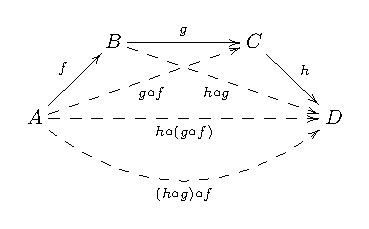
\includegraphics[scale=1.1]{doc/representation_matrix/representation_matrix.pdf}
	%	\label{fig:repr_mat}
	%	\caption{Map diagram of the representation matrix}
\end{figure}
The 'C' means that the diagram is commutative.

Since $\Phi^{-1}_{\mathcal{B}}, T, \Phi_{\mathcal{C}}$ are all linear maps, the map $\Phi_{\mathcal{C}} \circ T \circ \Phi^{-1}_{\mathcal{B}}: K^n \to K^m$ is also linear. By Lemma \ref{lem*mat_unique_lin_map}, any linear map $K^n \to K^m$ can be written using a matrix $A \in M_{m \times n}(K)$. In other words, there exists a unique matrix $A \in M_{m \times n}(K)$ s.t. $\Phi_{\mathcal{C}} \circ T \circ \Phi^{-1}_{\mathcal{B}} = T_A$. The matrix $A$ is called the \textbf{representation matrix of T w.r.t. the bases $\mathcal{B}$ and $\mathcal{C}$}. We denote this matrix by $[T]^{\mathcal{B}}_{\mathcal{C}} \in M_{m \times n}(K)$.

\subsubsection{Entries of the Representation Matrix}
Let $T:V \to W$ be a linear map and $\mathcal{B} = (v_1, \hdots , v_n)$ a basis for $V$, and $\mathcal{C} = (w_1, \hdots , w_m)$ a basis for $W$.
\begin{figure}[H]
	\centering
	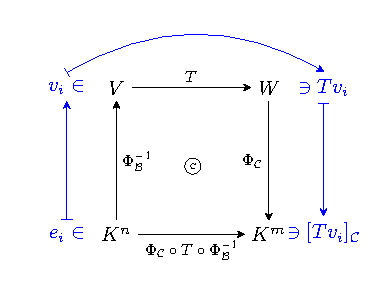
\includegraphics[scale=1.1]{doc/representation_matrix_2/representation_matrix_2.pdf}
\end{figure}
$T_A(e_i) = \Phi_{\mathcal{C}} \circ T \circ \Phi^{-1}_{\mathcal{B}}(e_i) = \Phi_{\mathcal{C}} \circ Tv_i = [Tv_i]_{\mathcal{C}}$. But these are precisely the columns of $A$. In other words
\[
A = [T]^{\mathcal{B}}_{\mathcal{C}} = \begin{pmatrix}
	\rule{0.5pt}{2ex} & & \rule{0.5pt}{2ex}\\
	[Tv_1]_{\mathcal{C}} & \hdots & [Tv_n]_{\mathcal{C}}\\
	\rule{0.5pt}{2ex} & & \rule{0.5pt}{2ex}\\
\end{pmatrix} \in M_{m\times n}.
\]
Another way to describe this matrix is: Let $A = (a_{i,j})$, where $a_{i,j}$ are defined uniquely by
\[
Tv_j = \sum_{i=1}^{m} a_{ij} w_j.
\]

\begin{proposition}{Represenation matrix}{repr_mat}
	Let $T:V \to W$ be a linear map between two finite dimensional vector spaces $V, W$. Let $\mathcal{B}, \mathcal{C}$ be bases for $V, W$ respectively. Then 
	\[
	\forall v \in V : \, [T]^{\mathcal{B}}_{\mathcal{C}} \cdot [v]_{\mathcal{B}} = [Tv]_{\mathcal{C}}.
	\]
\end{proposition}

\subsubsection{Representing Composition of Linear Maps by Matrices}
Let $T:V \to W, S:W \to U$ be linear maps. Let $\mathcal{A} = (v_1, \hdots , v_n)$ be a basis for $V$, $\mathcal{B} = (w_1, \hdots , w_m)$ a basis for $W$ and $\mathcal{C} = (u_1, \hdots , u_p)$ a basis for $U$.

Write $[T]^{\mathcal{A}}_{\mathcal{B}} = (a_{ij}), [S]^{\mathcal{B}}_{\mathcal{C}} = (b_{ij}), [S \circ T]^{\mathcal{A}}_{\mathcal{C}} = (c_{ij})$. By definition we have that
\begin{align}
	\label{eq:comp_mat_a}
	T(v_j) &= \sum_{k=1}^{m} a_{kj} w_k \qquad \forall 1 \leq j \leq n\\
	\label{eq:comp_mat_b}
	T(w_j) &= \sum_{i=1}^{p} b_{ij} u_i \qquad \forall 1 \leq j \leq m\\
	\label{eq:comp_mat_c}
	S \circ T(v_j) &= \sum_{i=1}^{p} c_{ij} u_i \qquad \forall 1 \leq j \leq n
\end{align}
But we can calculate $S \circ T(v_j)$ by using Equations \eqref{eq:comp_mat_a}, \eqref{eq:comp_mat_b}. Then we have
\begin{align*}
	S \circ T(v_j) &= S\big(\sum_{k=1}^{m} a_{kj} w_k\big) = \sum_{k=1}^{m} a_{kj} S(w_j) = \sum_{k=1}^{m} a_{kj} \big(\sum_{i=1}^{p}b_{ik} u_i \big)\\
	&= \sum_{k=1}^{m}\sum_{i=1}^{p} a_{kj}b_{ik} u_i = \sum_{i=1}^{p}\sum_{k=1}^{m} a_{kj}b_{ik} u_i = \sum_{i=1}^{p} \big(\sum_{k=1}^{m} b_{ik}a_{kj}\big) u_i\\
	\Longrightarrow \quad c_{ij} &= \sum_{k=1}^{m} b_{ik}a_{kj}.
\end{align*}

	% 
%
% (c) 2025 Autor, ETH Zürich
%
% !TEX root = linalg_I-II_summary.tex
% !TEX encoding = UTF-8
%

\section{Matrices}

\begin{definition}{Matrix Multiplication}{mat_mul}
	Let $A \in M_{m \times n}(K), B \in M_{n \times p}(K)$. We define a new matrix $A \cdot B \in M_{m \times p}(K)$ which is called the product of $A$ and $B$. Write $A = (a_{ij}), B = (b_{ij})$. The matrix $A \cdot B$ has entries $(c_{ij})$, where
	\[
	c_{ij} = \sum_{k=1}^{n} a_{ik}b_{kj}.
	\]
	\textbf{Important:} $A \cdot B$ is defined only when the number of columns of $A$ equals the number of rows of $B$.
\end{definition}

\textbf{Conclusion:} Let $T:V \to W, S:W \to U$ be lineear maps between finite dimensional vector spaces. Let $\mathcal{A}, \mathcal{B}, \mathcal{C}$ be bases for $V, W, U$ respectively. Then
\[
[S \circ T]^{\mathcal{A}}_{\mathcal{C}} = [S]^{\mathcal{B}}_{\mathcal{C}}\cdot [T]^{\mathcal{A}, \mathcal{B}}.
\]

\begin{definition}{Kronecker-Delta/Identity Matrix}{kron_delta}
	Let $\mathcal{I}$ be an index set. Define for all $i, j \in \mathcal{I}$
	\[
	\delta_{ij} := \begin{cases}
		1 & \text{if }i = j,\\
		0 & \text{if }i \neq j.
	\end{cases}
	\]
	This is called the \textbf{kronecker-delta}.
	
	We define the \textbf{identity matrix} $I_n \in M_{n \times n}(K)$ as
	\[
	I_n := \delta_{ij}, \qquad I_n = \begin{pmatrix}
		1 & \hdots & 0\\
		\vdots & \ddots & \vdots \\
		0 & \hdots & 1
	\end{pmatrix}.
	\]
\end{definition}

\begin{remark}
	Let $V$ be a finite dimensional vector space and $n := \dim V$. Let $id:V \to V$ be the identity map. Let $\mathcal{B}$ be any basis for $V$. Then $[id]^{\mathcal{B}}_\mathcal{B} = I_n$. In other words, the matrix representation of the identity map w.r.t $\mathcal{B} \& \mathcal{B}$ is the identity matrix $I_n$.
\end{remark}

\begin{proposition}{Associativity and Distributivity of Matrix Multiplication}{assoz_distr_mat_mul}
	\begin{enumerate}
		\item $\forall A \in M_{m \times n}(K), B \in M_{n \times p}(K), C \in M_{p \times q}(K) :\; (A B) C = A (B C) \in M_{m \times q}$.
		\item $\forall A,B \in M_{m \times n}(K), C \in M_{n \times p}(K), C' \in M_{q \times m}(K)$ we have
		\begin{align*}
			(A + B) C &= AC + BC \in M_{m \times p}(K),\\
			C' (A + B) &= C'A + C'B \in M_{q \times n}(K).
		\end{align*}
		\item $\forall A \in M_{m \times n}(K) : \; I_m A = A I_n = A$.
		\item $\forall \alpha \in K, A \in M_{m \times n}(K), B \in M_{n \times p}(K) : \; \alpha (A B) = (\alpha A) B = A (\alpha B)$.
	\end{enumerate}
\end{proposition}

\begin{remark}
	Matrix multiplication is in general \textbf{not} commutative, i.e., $\exists A, B$ s.t. $A B \neq B A$.
	
	In $M_{n \times n}(K)$ we can add/subtract matrices and also multiply matrices. There is also a unit $I_n$. These operations satisfy properties like associativity, distributivity, etc. From thsi we get that $M_{n \times n}(K)$ is a (non-commutative) \textbf{ring} with a unity.
\end{remark}

\begin{definition}{Invertibility}{inv}
	An $n \times n$ matrix $A \in M_{n \times n}(K)$ is \textbf{invertible} if $\exists B \in M_{n \times n}(K)$ s.t. $AB = BA = I_n$.
\end{definition}

\begin{remark}
	If $A$ is invertible, then there exists only one matrix $B$ s.t. $AB = BA = I_n$.
\end{remark}

\begin{proof}
	Assume $AB = BA = I_n$ and $AC = CA = I_n$. Then
	\[
	B = B I_n = B (AC) = (BA) C = I_n C = C.
	\qedhere
	\]
\end{proof}

\begin{definition}{The Inverse Matrix}{inv_mat}
	If $A$ is invertible, the unique matrix $B$ s.t. $AB = BA = I_n$ is called \textbf{the inverse of} $A$ and is denoted by $A^{-1}$. So, we have $A A^{-1} = A^{-1} A = I_n$.
	
	We denote the set of all invertible $n \times n$ matrices by
	\[
	GL_n(K) = GL(n, K) := \{A \in M_{n \times n}(K) \; |\; A \text{ is invertible}\}.
	\]
	This set is called the general linear group.
\end{definition}

\begin{proposition}{Structure of the General Linear Group}{struc_gl}
	$GL_n(K)$, endowed with matrix multiplication $(A, B) \mapsto A \cdot B$ is a group. The unity is $I_n$. The inverse of $A \in GL_n(K)$ is $A^{-1}$. Moreover, \[
	\forall A,B \in GL_n(K) :\; (A^{-1})^{-1} = A, \quad (AB)^{-1} = B^{-1}A^{-1}.
	\]
\end{proposition}

\begin{corollary}{Unique Solution for Linear System of Equations}{sol_lin_eq}
	Let $A \in GL_n(K)$. Then $\forall b \in K^n$ the linear system of equations $A  x = b$ has a unique solution, namely $x = A^{-1}b$.
\end{corollary}

\begin{proposition}{Invertibility and Isomorphisms}{inv_iso}
	Let $A \in M_{n \times n}(K)$. Then $A \in GL_n(K)$ if and only if $T_A:K^n \to K^n$ is an isomorphism. Moreover, $(T_A)^{-1} = T_{A^{-1}}$.
\end{proposition}

\begin{definition}{Upper/Lower Triangular and Diagonal Matrices}{triang_diag_mat}
	A matrix $A \in M_{n \times n}(K), A = (a_{ij})$, is called
	\begin{itemize}
		\item[$\bullet$] \textbf{Upper triangluar} if $a_{ij} = 0 \quad \forall i > j$, i.e.,
		\[
		\begin{pmatrix}
			\ast & \hdots & \hdots & \ast\\
			0 & \ddots & & \vdots \\
			\vdots & \ddots & \ddots & \vdots\\
			0 & \hdots & 0 & \ast 
		\end{pmatrix}.
		\]
		\item[$\bullet$] \textbf{Lower Triangular} if $a_{ij} = 0 \quad \forall i < j$, i.e.,
		\[
		\begin{pmatrix}
			\ast & 0 & \hdots & 0\\
			\vdots & \ddots & & \vdots \\
			\vdots & \ddots & \ddots & 0\\
			\ast & \hdots & \hdots & \ast		
		\end{pmatrix}.
		\]
		\item[$\bullet$] \textbf{Diagonal} if $a_{ij} = 0 \quad \forall i \neq j$, i.e.,
		\[
		\begin{pmatrix}
			1 & \hdots & 0\\
			\vdots & \ddots & \vdots\\
			0 & \hdots & 1
		\end{pmatrix}.
		\]
	\end{itemize}
\end{definition}

\begin{lemma}{Multiplication of Triangular/Diagonal Matrices}{mult_triang_diag_mat}
	Let $A, B$ be two diagonal (respectively both upper triangular, respectively both lower triangular). Then $A \cdot B$ is of the same type.
\end{lemma}

\begin{corollary}{Change of Bases for a Linear Map}{change_base_lin_map}
	Let $V, W$ be finite dimensional vector spaces over $K$. Let $n:= \dim V, m := \dim W$. Let $\mathcal{B}, \mathcal{B'}$ be two bases for $V$, and $\mathcal{C}, \mathcal{C'}$ be two bases for $W$. Then
	\begin{align*}
		[id_V]^{\mathcal{B'}}_{\mathcal{B}} &\in GL_n(K),\; [id_W]^{\mathcal{C}}_{\mathcal{C'}} \in GL_m(K), \text{and } \\ [id_V]^{\mathcal{B'}}_{\mathcal{B}} &= ([id_V]^{\mathcal{B}}_{\mathcal{B'}})^{-1},
		[id_V]^{\mathcal{C'}}_{\mathcal{C}} = ([id_V]^{\mathcal{C}}_{\mathcal{C'}})^{-1}.
	\end{align*}
	Let $T:V \to W$ be a linear map. Then
	\[
	[T]^{\mathcal{B'}}_{\mathcal{C'}} = [id_W]^{\mathcal{C}}_{\mathcal{C'}} \cdot [T]^{\mathcal{B}}_{\mathcal{C}} \cdot [T]^{\mathcal{B'}}_{\mathcal{B}}.
	\]
\end{corollary}

\begin{definition}{Transition Matrix/Change of Bases Matrix}{transition_change_mat}
	Let $V$ be a finite dimensional vector space over $K$, $n:= \dim V$. Let $\mathcal{B}, \mathcal{B'}$ be two bases of $V$. The matrix $[id_V]^{\mathcal{B}}_{\mathcal{B'}} \in GL_n(K)$ is called the \textbf{change of bases matrix} between $\mathcal{B}$ and $\mathcal{B'}$, or the \textbf{transition matrix} from basis $\mathcal{B}$ to basis $\mathcal{B'}$.
	
	If $\mathcal{B} = (v_1, \hdots , v_n), \mathcal{B'} = (v_1', \hdots , v_n')$ then
	\[
	[id_V]^{\mathcal{B}}_{\mathcal{B'}} = \begin{pmatrix}
		\rule{0.5pt}{2ex} & & \rule{0.5pt}{2ex}\\
		[v_1]_{\mathcal{B'}} & \hdots & [v_n]_{\mathcal{B'}}\\
		\rule{0.5pt}{2ex} & & \rule{0.5pt}{2ex}\\
	\end{pmatrix}.
	\]
\end{definition}

\begin{proposition}{Inverse of a Matrix with Bases}{inv_mat_bases}
	Let $T:V \to W$ bw an isomorphism between two finite dimensional vector spaces. Let $\mathcal{B}, \mathcal{C}$ be bases for $V, W$ respectively. Then $[T]^{\mathcal{B}}_{\mathcal{C}}$ is an invertible matrix and
	\[
	[T^{-1}]^{\mathcal{C}}_{\mathcal{B}} = ([T]^{\mathcal{B}}_{\mathcal{C}})^{-1}.
	\]
\end{proposition}

\begin{corollary}{Change of Basis for an Endomorphism}{change_base_endo}
	Let $V$ be a finite dimensional vector space and $T:V \to V$ a linear map (an endomorphism). Let $\mathcal{B}, \mathcal{B'}$ be two bases for $V$. Then
	\[
	[T]^{\mathcal{B'}}_{\mathcal{B'}} = [id_V]^{\mathcal{B}}_{\mathcal{B'}} \cdot [T]^{\mathcal{B}}_{\mathcal{B}} \cdot [id_V]^{\mathcal{B'}}_{\mathcal{B}} = ([id_V]^{\mathcal{B'}}_{\mathcal{B}})^{-1} \cdot [T]^{\mathcal{B}}_{\mathcal{B}} \cdot [id_V]^{\mathcal{B'}}_{\mathcal{B}}.
	\]
\end{corollary}

\begin{definition}{Equivalence and Similarity of Matrices}{equiv_sim_mat}
	\begin{enumerate}
		\item Let $A, B \in M_{m \times n}(K)$. We say that $A$ and $B$ are \textbf{equivalent} if $\exists\, P \in GL_m(K), Q \in GL_n(K)$ s.t. $B = PAQ$.
		\item Let $A, B \in M_{n \times n}(K)$. We say that $A$ and $B$ are \textbf{similar} if $\exists\, P \in GL_n(K)$ s.t. $B = P^{-1} A P$.
	\end{enumerate}
\end{definition}

\begin{remark}
	\begin{enumerate}
		\item Equivalence between $m \times n$ matrices gives an equivalence relation on $M_{m \times n}(K)$.
		\item $A, B \in M_{m \times n}(K)$ are equivalent if and only if there exists two vector spaces $V, W$ with $n:= \dim V$, $m := \dim W$ and two bases $\mathcal{B}, \mathcal{B'}$ of $V$ and two bases $\mathcal{C}, \mathcal{C'}$ for $W$ s.t. $A = [T]^{\mathcal{B}}_{\mathcal{C}}$, $B = [T]^{\mathcal{B'}}_{\mathcal{C'}}$. In other words, $A$ is equivalent to $B$ if and only if $A$ and $B$ are matrix representations of the same linear map w.r.t. different choices of bases for $V$ and $W$.
		\item Similarity between $n \times n$ matrices gives an equivalence relation on $M_{n \times n}(K)$.
		\item $M,N \in M_{n \times n}(K)$ are similar if and only if there exists and $n$-dimensional vector space $V$ and $T:V \to V$ and two bases $\mathcal{B}, \mathcal{B'}$ of $V$ s.t. $M = [T]^{\mathcal{B}}_{\mathcal{B}}$, $N = [T]^{\mathcal{B'}}_{\mathcal{B'}}$.
	\end{enumerate}
\end{remark}

\begin{proposition}{Existence of 'Nice' Bases}{exist_nice_bases}
	Let $V, W$ be finite dimensional vector spaces over $K$, of dimension $n := \dim V$, $m := \dim W$. Let $T:V \to W$ be a linear map with $\operatorname{rank}(T) = r$. (Recall that $\operatorname{rank}(T) := \dim \operatorname{Im}(T)$.) Then there exists a basis $\mathcal{B} = (v_1, \hdots , v_n)$ of $V$ and a basis $\mathcal{C} = (w_1, \hdots , w_m)$ of $W$ s.t.
	\[
	[T]^{\mathcal{B}}_{\mathcal{C}} = \begin{pmatrix}
		I_r & 0_{r, n-r}\\
		0_{m-r, r} & 0_{m-r, n-r}
	\end{pmatrix}.
	\]
\end{proposition}

\begin{corollary}{}{cor_exist_nice_bases}
	Let $A \in M_{m \times n}(K)$. Then $\exists P \in GL_m(K), Q \in GL_n(K)$ s.t.
	\[
	PAQ = \begin{pmatrix}
		I_r & 0_{r, n-r}\\
		0_{m-r, r} & 0_{m-r, n-r}			
	\end{pmatrix},
	\]
	where $r = \operatorname{col-rank}(A)$. In particular, $\operatorname{col-rank}(A) \leq \min\{m,n\}$.
\end{corollary}

\begin{corollary}{Condition for Equivalence if Matrices}{cond_equiv_mat}
	Let $A, B \in M_{m \times n}(K)$. Then $A \sim B$ if and only if $\operatorname{col-rank}(A) = \operatorname{col-rank}(B)$. 
	
	Moreover, $\forall\, 0 < r \leq \min\{m, n\}$ there is precisely one equivalence class of matrices $A$ with $\operatorname{col-rank} = r$.
\end{corollary}

\subsection{col-rank = row-rank}

\begin{theorem}{col-rank = row-rank}{colrank_rowrank}
	Let $A \in M_{m \times n}(K)$. Then $\operatorname{col-rank}(A) = \operatorname{row-rank}(A)$.
\end{theorem}

\begin{remark}
	\begin{enumerate}
		\item Because of this Theorem we'll denote from now on $\operatorname{rank}(A) := \operatorname{col-rank}(A) = \operatorname{row-rank}(A)$.
		\item Suppose $A'$ is a row-reduced echelon matrix which is row-equivalent to $A$. Then we have that $\operatorname{rank}(A) =$ \# pivots in $A'$. Indeed, $\operatorname{rank}(A) = \operatorname{row-rank}(A) = \operatorname{row-rank}(A') =$ \# pivots in $A'$.
		\item Recall that for $T:V \to W$ we defined $\operatorname{rank}(T) := \dim \operatorname{Im}(T)$. Also, if $A \in M_{m \times n}(K)$, then $\operatorname{rank}(T_A) = \dim \operatorname{Im}(T) = \operatorname{col-rank}(A)$.
	\end{enumerate}
\end{remark}

We now present some Lemmas for the proof of the Theorem.

\begin{lemma}{Isomorphisms preserve the Rank}{iso_preserve_rank}
	Let $T:V \to W$ be a linear map, and $S:W \overset{\cong}{\longrightarrow} U$, $L: P \overset{\cong}{\longrightarrow} V$ be isomorphisms. Then
	\begin{enumerate}
		\item $\operatorname{rank}(S \circ T) = \operatorname{rank}(T)$.
		\item $\operatorname{rank}(T \circ S) = \operatorname{rank}(T)$.
	\end{enumerate}
\end{lemma}

\begin{lemma}{}{lemma_2}
	Let $A\in M_{m \times n}(K)$. Then $A$ is invertible if and only if $T_A K^n \to K^n$ is in isomorphism.
\end{lemma}

\begin{lemma}{Equivalent Matrices Have the Same Rank}{equiv_same_rank}
	Let $A, B \in M_{m\times n}(K)$ s.t. $B = PAQ$, where $P \in GL_m(K)$, $Q \in GL_m(K)$. Then
	\begin{enumerate}
		\item $\operatorname{col-rank}(A) = \operatorname{col-rank}(B)$
		\item $\operatorname{row-rank}(A) = \operatorname{row-rank}(B)$.
	\end{enumerate}
\end{lemma}

\begin{proof}
	\textbf{Proof of Theorem \ref{theo*colrank_rowrank}:} By Corollary \ref{cor*cor_exist_nice_bases}, $\exists P \in GL_m(K), Q \in GL_n(K)$ s.t. 
	\[
		PAQ = \begin{pmatrix}
			I_r & 0_{r, n-r}\\
			0_{m-r, r} & 0_{m-r, n-r}
		\end{pmatrix}.
	\]
	Denote this matrix by $B$. For $B$ we have $\operatorname{col-rank}(B) = \operatorname{row-rank}(B) = r$. By Lemma \ref{lem*equiv_same_rank}, we have that $\operatorname{col-rank}(A) = \operatorname{col-rank}(B) = r$, and $\operatorname{row-rank}(A) = \operatorname{row-rank}(B) = r$. Therefore, $\operatorname{col-rank}(A) = \operatorname{row-rank}(A)$. \qedhere
\end{proof}

\begin{remark}
	Although $\operatorname{row-rank}(A) = \operatorname{col-rank}(A)$, the spaces $\operatorname{ColS}(A)$ and $\operatorname{RowS}(A)$ are \textbf{different}. First of all if $A \in M_{m \times n}$, then $\operatorname{ColS}(A) \subseteq K^m$ and $\operatorname{RowS}(A) \subseteq K^n$. But even when $n = m$, these two spaces are \textbf{different}. They have the same dimension, but are different.
\end{remark}


\subsection{More on Matrices and Linear Equations}
Let $A \in M_{m \times n}(K)$, and consider the system of linear equations $A x = 0$. Denote by
\[
	\operatorname{Sol}(A,0) := \{x \in K^n \;|\; Ax = 0\} = \ker(T_A),
\]
the \textbf{space} of solutions $Ax = 0$. Note that $\dim \operatorname{Sol}(A,0) = n - \operatorname{rank}(A)$ (b.c. $\dim \ker(T_A)) = n - \dim \operatorname{Im}(T_A)$). Let $A'$ be a row-reduced echelon matrix which is row-equivalent to $A$ (e.g. $A'$ is obtained from $A$ by Gauss-elimination). \# pivots of $A'$ = $\operatorname{rank}(A)$, $n - \operatorname{rank}(A) =$ \# free variables. Also, we have that $\operatorname{Sol}(A,0) = \operatorname{Sol}(A', 0)$.
\[
	\begin{pmatrix}
		0 & \hdots & 0 & 1 & \ast & \hdots & \ast \\
		0 & \hdotsfor{3} & 0 & 1 & \ast & \hdots & \ast \\
		0 & \hdotsfor{4} & 0 & 1 & \ast & \hdots & \ast \\
		0 & \hdotsfor{8} & 0\\
		0 & \hdotsfor{8} & 0 
	\end{pmatrix}
	\begin{pmatrix}
		x_1\\
		\vdots \\
		x_n
	\end{pmatrix}
	=
	\begin{pmatrix}
		0\\
		\vdots \\
		0
	\end{pmatrix}.
\]
Denote by $x_{i_1}, \hdots , x_{i_l}$ the free variables, where $1 \leq i_1 < \hdots < i_l \leq n$, $l = n - \operatorname{rank}(A)$ and by $x_{j_1}, \hdots , x_{j_k}$, where $1 \leq j_1 < \hdots < j_k \leq n$, $r = \operatorname{rank}(A)$ the pivots. For each choice of values for the free variables $x_{i_1}, \hdots , x_{i_l} \in K$, the pivot variables $x_{j_1}, \hdots , x_{j_k}$ are uniquely determined. So, we obtain a map
\begin{align*}
	\Phi: K^l &\to \operatorname{Sol}(A,0)\\
	\Phi(\lambda_1 ,\hdots , \lambda_l) &= \text{ the unique solution of } Ax = 0,
\end{align*}
with $x_{i_1} = \lambda_1, \hdots , x_{i_l} = \lambda_l$.

\begin{proposition}{$\Phi$ is an Isomorphism}{phi_iso}
	The map $\Phi$ is linear. Moreover, it is an isomorphism.
\end{proposition}

\begin{corollary}{}{cor_phi}
	Let $b \in K^m$, $A \in M_{m \times n}(K)$. Then
	\begin{enumerate}
		\item $\operatorname{Sol}(A, b) := \{x \in K^n \;|\; Ax = b\} \neq \emptyset$ iff $b \in \operatorname{ColS}(A)$.
		\item If $\operatorname{Sol}(A, b) \neq \emptyset$ and $y \in \operatorname{Sol}(A, b)$ then
		\[
			\operatorname{Sol}(A,b) = y + \operatorname{Sol}(A,0) := \{y + x \;|\; x \in \operatorname{Sol}(A, 0)\}.
		\] 
	\end{enumerate}
\end{corollary}

\begin{proposition}{}{prop_phi}
	Let $A \in M_{m \times n}(K)$, $b \in K^m$. The following statements are equivalent:
	\begin{enumerate}
		\item $\operatorname{rank}(A | b) = \operatorname{rank}(A)$.
		\item The system of equations $Ax = b$ has a solution.
	\end{enumerate}
\end{proposition}

\begin{proposition}{}{prop_phi_2}
	\begin{enumerate}
		\item $\operatorname{rank}(A | b) = \operatorname{rank}(A) = n$.
		\item The system of equations $Ax = b$ has a unique solution.
	\end{enumerate}
\end{proposition}

\subsection{Elementary Row Operations Revisited}
Let $A \in M_{n \times p}(K)$. We learned about elementary row operations which are used as part of the Gauss elimination. All of these operations can be expressed by matrix multiplications.

Denote by $E_{ij}$ the matrix in Example \ref{exp:bases}.

\begin{itemize}
	\item[\textbf{Type I:}] Let $1 \leq i \leq n$, $1 \leq j \leq n$, $i \neq j$. Let $\alpha \in K$. Define $Q_{ij}(\alpha)$ to be the matrix obtained from $I_n$ after applying $R_i + \alpha R_j \longrightarrow R_i$. We have $Q_{ij}(\alpha) = I_n + \alpha E_{ij}$.
	
	\item[\textbf{Type II:}] Let $1 \leq i \leq n, 1 \leq j \leq n$. Define $P_{ij}$ to be the matrix obtained from $I_n$ by permuting (exchanging) row \# i and row \# j, i.e. applying $R_i \longleftrightarrow R_j$. We have $P_{ij} = I_n - E_{ii} - E_{jj} + E_{ij} + E_{ji}$.
	\item[\textbf{Type III:}] Let $1 \leq i \leq n$ and $0 \neq \alpha \in K$. Denote by $S_i(\alpha)$ the matrix obtained from $I_n$ by applying $\alpha R_i \longrightarrow R_i$.
\end{itemize}

\begin{lemma}{Elementary Row Operations as Matrix Multiplication}{row_op_mat_mul}
	Let $A \in M_{n \times p}(K)$. 
	\begin{enumerate}
		\item Multiplying $A$ from the left with $Q_{ij}(\alpha)$ results in the row operation $R_i + \alpha R_j \longrightarrow R_i: \, A \overset{R_i + \alpha R_j \to R_i}{\rightarrow} Q_{ij}(\alpha) A$.
		\item Multiplying $A$ from the left with $P_{ij}$ results in the row operation $R_i \longleftrightarrow R_j: \, A \overset{R_i \leftrightarrow R_j}{\longrightarrow} P_{ij} A$.
		\item Multiplying $A$ from the left with $S_i(\alpha)$ results in the row operation $\alpha R_i \longrightarrow R_i: \, A \overset{\alpha R_i \to R_i}{\longrightarrow} S_i(\alpha) A$.
	\end{enumerate}
	The same holds for elementary column operations, which is done by right hand side multiplications of the matrices.
\end{lemma}

\begin{lemma}{Elementary Matrices are Invertible}{elem_mat_inv}
	Every elementary matrix is invertible, and the inverse of each of them is an elementary matrix of the same type, i.e.
	\[
		Q_{ij}(\alpha)^{-1} = Q_{ij}(-\alpha), \qquad P_{ij}^{-1} = P_{ji}, \qquad S_{ij}(\alpha )^{-1} = S_{ij}(\alpha ^{-1}).
	\]
\end{lemma}

\begin{theorem}{}{elem_mat_thm}
	$\forall \, A \in GL_n(K), \; \exists\, k \geq 1$ and elementary matrices $T_1, \hdots , T_k$ s.t. $T_k\cdot \hdots \cdot T_1 \cdot A = I_n$. Furthermore, we have that
	\[
		A = T_1^{-1}\cdot \hdots \cdot T_k^{-1}, \qquad A^{-1} = T_k\cdot \hdots \cdot T_1.
	\]
	In particular, $A$ can be written as a finite product of elementary matrices.
\end{theorem}

\begin{theorem}{Equivalent condition for Invertibility}{equiv_cond_inv}
	Let $A \in M_{n \times n}(K)$. Place $A$ together with $I_n$ in the following way $(A | I_n)$. Then $A$ is invertible if and only if $(A | I_n)$ can be brought via a sequence of elementary row-operations to the form $(I_n | B)$ for some matrix $B \in M_{n \times n}(K)$. In this case we have $A^{-1} = B$.
\end{theorem}






	% 
%
% (c) 2025 Autor, ETH Zürich
%
% !TEX root = linalg_I-II_summary.tex
% !TEX encoding = UTF-8
%

\section{Constructing New Vector Spaces Out of Old Ones}

\begin{proposition}{The Vector Space of Linear Functions}{vect_sp_lin_func}
	Let $V, W$ be two vector spaces over $K$. Then $\operatorname{Hom}(V, W)$ has the structure of a vector space over $K$, if we endow it with the following operations:
	\begin{itemize}
		\item[$\bullet$] $\forall \, T_1,T_2 \in \operatorname{Hom}(V, W), \; (T_1 + T_2)(v) := T_1(v) + T_2(v) \quad \forall \, v \in V$.
		\item[$\bullet$] $\forall \, T \in \operatorname{Hom}(V, W), \alpha \in K, \; (\alpha T)(v) := \alpha T(v) \quad \forall \, v \in V$.
	\end{itemize}
	The neutral element of $\operatorname{Hom}(V, W)$ is the map $0: V\to W, \quad v \mapsto 0$.
\end{proposition}

\begin{theorem}{The map $\Psi^{\mathcal{B}}_{\mathcal{C}}$}{map_psi}
	Let $V, W$ be finite dimensional vector spaces over $K$, $\mathcal{B} = (v_1 , \hdots , v_n)$ a basis for $V$, and $\mathcal{C} = (w_1, \hdots , w_n)$ a basis for $W$. Then the map
	\[
		\Psi^{\mathcal{B}}_{\mathcal{C}}: \operatorname{Hom}(V, W) \to M_{m \times n}(K)
	\]
	defined by
	\[
		T \mapsto [T]^{\mathcal{B}}_{\mathcal{C}} := \begin{pmatrix}
			\rule{0.5pt}{2ex} & & \rule{0.5pt}{2ex}\\
			[Tv_1]_{\mathcal{C}} & \hdots & [Tv_n]_{\mathcal{C}}\\
			\rule{0.5pt}{2ex} & & \rule{0.5pt}{2ex}\\
		\end{pmatrix}
	\]
	is a linear map and moreover an isomorphism.
\end{theorem}

\begin{corollary}{Dimesnion of $\operatorname{Hom}(V, W)$}{dim_hom}
	If $V, W$ are finite dimensional vector spaces then so is $\operatorname{Hom}(V, W)$ and $\dim \operatorname{Hom}(V, W) = \dim V \cdot \dim W$.
\end{corollary}

\subsubsection{Rings}
Recall that Rings have the same axioms as Fields except that we do \textbf{not} require that every non-zero element has an inverse.

\begin{definition}{Homomorphism of Rings}{homo_ring}
	Let $R, S$ be rings. A \textbf{homomorphism of rings} is a map $\varphi: R \to S$ s.t.:
	\begin{itemize}
		\item[$\bullet$] $\forall \, r_1,r_2 \in R : \, \varphi(r_1 + r_2) = \varphi(r_1) + \varphi(r_2)$.
		\item[$\bullet$] $\forall \, r_1,r_2 \in R: \, \varphi(r_1 \cdot r_2) = \varphi(r_1) \cdot \varphi(r_2)$
		\item[$\bullet$] $\varphi(1) = 1$.
		\item[$\bullet$] $\varphi(0) = 0$.
	\end{itemize}
\end{definition}

\begin{corollary}{$\Psi$ for an Endomorphism is an isomorphism of Rings}{endo_homo_ring}
	Let $V$ be a vector space over $K$. Then $\operatorname{End}(V) := \operatorname{Hom}(V, V)$ is a ring with a unity. This ring is, in general, not commutative. The multiplication (product) in $\operatorname{End}(V)$ is given by composition, i.e.,
	\[
		T_1 \cdot T_2 := T_1 \circ T_2 \qquad \forall \, T_1, T_2 \in \operatorname{Hom}(V,V).
	\]
	The unity is $id_V$. Moreover, if $V$ is finite dimensional and $\dim V = n$, and $\mathcal{B} = (v_1, \hdots , v_n)$ is a basis for $V$, then $\Psi^{\mathcal{B}}_{\mathcal{B}}: \operatorname{Hom}(V,V) \to M_{n \times n}(K)$ is an isomorphism of rings
\end{corollary}

\subsection{Dual Space}
An important special case of $\operatorname{Hom}(V,W)$ is when $W = K$.

\begin{definition}{Dual Space}{dual_sp}
	Let $V$ be a vector space over $K$. The \textbf{dual space} of $V$, is defined to be the vector space $V^* := \operatorname{Hom}(V,K)$. The elements of $V^*$ are linear maps $\ell :V \to K$, and are sometimes called \textbf{functionals} (on $V$).
\end{definition}

\begin{corollary}{Dimension of the Dual Space}{dim_dual_sp}
	Let $V$ be a finite dimensional vector space over $K$. Then $\dim V^* = \dim V$.
\end{corollary}

Let $V = K^n_{\text{col}}$. Then we can identify $V^*$ with $K^n_{\text{col}}$, as follows: If $\ell \in K^n_{\text{row}}$, then $\ell$ defines a functional $f_{\ell}:K^n_{\text{col}} \to K$ by $f_{\ell}(v) := \ell \cdot v \in K$. The map $D:K^n_{\text{row}} \to (K^n_{\text{col}})^*$ defined by $D(\ell) := f_{\ell}$ is a linear map and is an isomorphism.

Let $V$ be a finite dimensional vector space over $K$ and $\mathcal{B} = (v_1, \hdots , v_n)$ a basis for $V$. $\forall \, 1 \leq i \leq n$, define a functional $v_i^* \in V^*$, i.e., $v_i^*:V \to K$ linear map, as follows:
\[
	v_i^*(v_j) := \delta_{ij} = \begin{cases}
		1 & i = j\\
		0 & i \neq j
	\end{cases}.
\]
Since $v_1, \hdots , v_n$ form a basis for $V$, our definition determines uniquely a well-defined functional $v_i^*:V \to K$.

\begin{lemma}{\textcolor{red}{The Dual Basis}}{dual_base}
	The elements $v_1^*, \hdots , v_n^* \in V^*$ form a basis for $V^*$. This basis is called the \textbf{dual basis} to $\mathcal{B}$. We denote this basis by $\mathcal{B}^* = (v_1^*, \hdots , v_n^*)$.
	
	Moreover,
	\[
		\forall \, \ell  \in V^* : \, \ell = \sum_{i=1}^{n} \ell(v_i)\cdot v_i^*.
	\] 
\end{lemma}

\begin{proof}
	Let $\ell \in V^*$. We claim that 
	\begin{equation}
		\label{eq:dual_1}
		\ell = \sum_{i=1}^{n} \ell(v_i) \cdot v_i^*.
	\end{equation}
	Or in other words, we claim that
	\begin{equation}
		\label{eq:dual_2}
		\forall \, v \in V: \, \ell(v) = \sum_{i=1}^{n} \ell(v_i) \cdot v_i^*(v).
	\end{equation}
	Indeed, both sides of Equation \eqref{eq:dual_1} are linear maps $V \to K$, so it's enough to check that Equation \eqref{eq:dual_2} holds for $v = v_1, \hdots , v = v_n$, b.c. $v_1, \hdots , v_n$ form a basis for $V$. And indeed, for $v = v_k$ we have
	\[
	\sum_{i=1}^{n} \ell(v_i)\cdot v_i^*(v_k) = \sum_{i=1}^{n} \ell(v_i)\cdot \delta_{ik} = \ell(v_k).
	\]
	The claim just proven shows that $v_1^*,\hdots , v_n^*$ span $V^*$. Since $\dim V^* = \dim V = n$, it follows that $v_1^*, \hdots , v_n^*$ form a basis for $V^*$.
\end{proof}

\textbf{Question:} Let $V$ be a finite dimensional vector space over $K$. Let $\mathcal{B}$ and $\mathcal{C}$ be two bases for $V$. Therefore, $\mathcal{B}^*$ and $\mathcal{C}^*$ are two bases for $V^*$. What is the relation between $[id_{V^*}]^{\mathcal{C}^*}_{\mathcal{B}^*}$ and $[id_V]^{\mathcal{C}}_{\mathcal{B}}$.

\begin{proposition}{Relation between $[id_{V^*}]^{\mathcal{C}^*}_{\mathcal{B}^*}$ and $[id_V]^{\mathcal{C}}_{\mathcal{B}}$}{rel_change_base}
	\[
		[id_{V^*}]^{\mathcal{C}^*}_{\mathcal{B}^*} = \big([id_V]^{\mathcal{B}}_{\mathcal{C}}\big)^T = \bigg(\big([id_V]^{\mathcal{C}}_{\mathcal{B}}\big)^T\bigg)^{-1}. 
	\]
\end{proposition}

\subsection{The Dual Map}
\label{sec:dual_map}

\begin{definition}{\textcolor{red}{The Dual Map}}{dual_map}
	Let $V, W$ be vector spaces over $K$. Let $T:V \to W$ be a linear map. Define a new map 
	\[
		T^*:W^* \to V^*, \quad T^*(\ell) = \ell  \circ T \quad \forall \, \ell \in W^*.
	\]
	Then $T^*$ is a linear map. It is called \textbf{the dual map} to $T$.
\end{definition}


\begin{proof}
	Let $\ell \in W^*$, i.e., $\ell :W \to K$ a linear map. Clearly
	\[
		\ell \circ T:V \to K
	\]
	is a linear map, b.c. both $\ell$ and $T$ are linear. So, $T^*(\ell) := \ell \circ T \in V^*$. This shows that $T^*:W^* \to V^*$ indeed has as it's target $V^*$ as claimed, see also the Figure \ref{fig:dual_map}.
	\begin{figure}[h]
		\label{fig:dual_map}
		\centering
		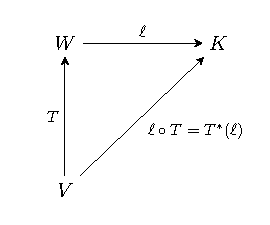
\includegraphics{doc/dual_map/dual_map.pdf}
		\caption{Map diagram of the dual map}
	\end{figure}
	We'll show now that $T^*$ is a linear map. Let $\ell \in W^*$, $\alpha \in K$. We have that $T^*(\alpha \ell) \in V^*$ is the map
	\begin{align*}
				T^*(\alpha \ell)(v) &= \big((\alpha \ell) \circ T\big)(v) = (\alpha \ell) (Tv) = \alpha \ell (Tv) = \alpha (\ell \circ T)(v) = \alpha \big(T^*(\ell)\big)(v)\\
				\Longrightarrow \qquad T^*(\alpha \ell) &= \alpha T^*(\ell).
	\end{align*}
	
	Now, let $\ell_1, \ell_2 \in W^*$. We have that $T^*(\ell_1 + \ell_2) \in V^*$ is the map
	\begin{align*}
		T^*(\ell_1 + \ell_2)(v) &= \big((\ell_1 + \ell_2) \circ T\big)(v) = (\ell_1 \circ T + \ell_2 \circ T)(v) = (\ell_1 \circ T)(v) + (\ell_2 \circ T)(v)\\
		&= \big(T^*(\ell_1)\big)(v) + \big(T^*(\ell_2)\big)(v) \\
		\Longrightarrow \qquad T^*(\ell_1 + \ell_2) &= T^*(\ell_1) + T^*(\ell_2).
	\end{align*}
	This shows that $T^*$ is linear as claimed. \qedhere
\end{proof}

\begin{proposition}{Composition of the Dual Map}{comp_dual_map}
	Let $U,V, W$ be vector spaces over $K$. Let $T:V \to W$, $S:W \to U$ be linear maps. Consider $T^*:W^* \to V^*$, $S^*:U^* \to W^*$, the dual maps. Then
	\[
		(S \circ T)^* = T^* \circ S^*.
	\]
\end{proposition}

\begin{lemma}{\textcolor{red}{Interpretation of the Matrix Transpose}}{int_mat_trans}
	Let $S:V \to W$ be a linear map between two finite dimensional vector spaces $V$ and $W$ over $K$. Let $\mathcal{B}$ be a basis for $V$ and $\mathcal{C}$ be a basis for $W$. Consider $S^*:W^* \to V^*$ and the bases $\mathcal{C}^*, \mathcal{B}^*$ for $W^*, V^*$ respectively. Then
	\[
		[S^*]^{\mathcal{C}^*}_{\mathcal{B}^*} = \big([S]^{\mathcal{B}}_{\mathcal{C}}\big)^T.
	\]
\end{lemma}

\begin{proof}
	Write $\mathcal{B} = (v_1, \hdots , v_n), \mathcal{C} = (w_1,\hdots , w_m)$. Define $A := [S]^{\mathcal{B}}_{\mathcal{C}}, A = (a_{ij})$. $A$ satisfies
	\[
		Sv_j = \sum_{i=1}^{m} a_{ij} w_i.
	\]
	Now, for $w_j^* \in \mathcal{C}^*$ we have by Lemma \ref{lem*dual_base}
	\begin{align*}
		S^*w_j^* &= w_j^* \circ S = \sum_{i=1}^{n} (w_j^* \circ S)(v_i) \cdot v_i^* = \sum_{i=1}^{n} w_j^*\big(S(v_i)\big)\cdot v_i^*\\
		&= \sum_{i=1}^{n}w_j^*\bigg(\sum_{k=1}^{m}a_{ki} w_k\bigg)\cdot v_i^* = 
		\sum_{i=1}^{n} \sum_{k=1}^{m} a_{ki} w_j^*(w_k) \cdot v_i^* =	\sum_{i=1}^{n} a_{ji} v_i^*.
	\end{align*}
	Therefore, the coordinates of $S^*w_j^*$ in the basis $\mathcal{B}^* = (v_1^*, \hdots , v_n^*)$ are
	\[
		\begin{pmatrix}
			a_{j1}\\
			\vdots \\
			a_{jn}
		\end{pmatrix},
	\]
	which is the row \#$j$ in $A$, represented as a column, or equivalently the column \#$j$ in the matrix $A^T$. \qedhere
\end{proof}

\subsection{Reflexitvity}
Let $V$ be a vector space over $K$. We have $V^*$, but also $V^{**} := (V^*)^*$ by applying 'dual' one more time, to $V^*$. $(V^*)^*$ is sometimes called the bidual space of $V$. Is there any relation between $(V^*)^*$ and $V$.

\begin{theorem}{The Canonical Isomorphism between $(V^*)^*$ and $V$}{canonic_iso_bidual}
	Let $v$ be a \textcolor{red}{finite} dimensional vector space over $K$. Then there exists a canonical isomorphism $\tau: V \to (V^*)^*$, given by
	\[
		\forall \, v \in V, \; \tau(v):V^* \to K
	\]
	is the map
	\[
		\tau(v)(\ell) := \ell(v) \quad \forall \, \ell \in V^*.
	\]
	In other words,
	\[
		V \owns v \overset{\tau}{\longmapsto} \big(V^*\owns \ell \longmapsto \ell(v) \in K\big).
	\]
\end{theorem}

\begin{remark}
	The map $\tau:V \to (V^*)^*$ exists and is defined in the same way as above regardless of $V$ being finite or infinite dimensional. Moreover, $\tau$ is always injective. However, when $V$ is infinite dimensional, $\tau$ fails to be surjective.
\end{remark}

\subsection{Naturality}
The map $\tau: V \to (V^*)^*$ exists for every space $V$, and is defined in the same way. To distinguish $\tau$'s for different spaces, denote it now by $\tau_V:V \to (V^*)^*$. Let $V, W$ be two vector spaces over $K$. Then for every linear map $T: V \to W$ we have
\begin{figure}[H]
	\centering
	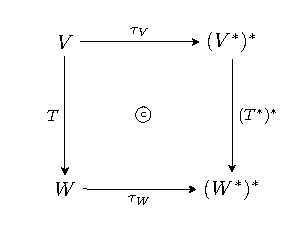
\includegraphics{doc/naturality/naturality.pdf}
\end{figure}
which we call naturality.

\begin{proposition}{Image of $\tau$}{img_tau}
	Let $V$ be a finite dimensional vector space over $K$, let $\mathcal{B} = (V_1,\hdots , v_n)$ be a basis for $V$. Let $\mathcal{B}^* = (v_1^*, \hdots , v_n^*)$ be the dual basis and $(\mathcal{B}^*)^* = ((v_1^*)^*,\hdots , (v_n^*)^*)$ the basis for $(V^*)^*$, which is dual to $\mathcal{B}^*$. Then $\tau(\mathcal{B}) = (\mathcal{B}^*)^*$, i.e.,
	\[
		\tau(v_i) = (v_i^*)^* \qquad \forall \, 1 \leq i \leq n.
	\]
\end{proposition}

\subsection{Direct Sums}

\begin{proposition}{The Vector Space of the Cartesian Product}
	Let $V, W$ be a vector space over $K$. Then the cartesian product $V \times W$ becomes a vector space over $K$ if we endow it with the following operations:
	\begin{itemize}
		\item[$\bullet$] $\forall \, (v_1, w_1), (v_2, w_2) \in V \times W : \; (v_1, w_1) + (v_2, w_2) := (v_1+v_2, w_1+ w_2)$.
		\item[$\bullet$] $\forall \, \alpha \in K, (v,w) \in V \times W : \; \alpha \cdot (v,w) := (\alpha v, \alpha w) \in V \times W$.
		\item[$\bullet$] $0_{V \times W} := (0_V, 0_W)$.
	\end{itemize}
	This new vector space $V \times W$ is usually denoted $V \oplus W$ and is called the direct sum of $V$ and $W$. We write the elements of $V \oplus W$ as $(v,w)$ or $v \oplus w$.
\end{proposition}

\begin{remark}
	$V \oplus W$ comes together with the following \textbf{canonical maps}:
	\begin{enumerate}
		\item[\textcolor{blue}{1)}] $i_V:V \to V \oplus W, \quad i_V(v) := (v,0)$.
		\item[\textcolor{blue}{2)}] $i_W:W \to V \oplus W, \quad i_W(w) := (0,w)$.
		\item[\textcolor{orange}{3)}] $p_V:V \oplus W \to V, \quad p_V(v,w) := v$.
		\item[\textcolor{orange}{4)}] $p_W:V \oplus W \to W, \quad p_W(v,w) := w$.
	\end{enumerate}
	The blue marked maps are canonical embeddings, while the orange marked maps are canonical projections.
	These maps are all linear. The maps $p_V, p_W$ are surjective, and $i_V, i_W$ are injective. Becuase of the maps $i_V, i_W$ we can sometimes view $V$ and $W$ as subspaces of $V \oplus W$.
\end{remark}

\begin{proposition}{The map $\varphi$}{map_phi}
	Let $V$ be a vector space over $K$, $U \subseteq V$ a subspace and $U' \subseteq V$ another subspace which is a complement of $U$ in $V$ (recall Definition \ref{def*lin_compl}). Then the map
	\[
		\varphi: U \oplus U' \to V, \quad \varphi(u, u') := u + u'
	\]
	is a linear isomorphism.
\end{proposition}

\begin{remark}
	When $U'$ is a complement of $U$ in $V$, then $U+ U' = V$ and we also have a canonical isomorphism $U \oplus U' \overset{\cong}{\longrightarrow} V$. But formally speaking $U \oplus U'$ is a different vector space than $V$.
\end{remark}

\subsubsection{Generalization to more Summands}
Let $U_1, \hdots , U_m$ be \textbf{finitely} many vector spaces over $K$. We can define $U_1 \oplus \hdots \oplus U_m := U_1 \times \hdots \times U_m$, with the coordinatewise/componentwise operations.

For \textbf{infinite} families $U_i,\, i\in \mathcal{I}$ one can define
\[
	\bigoplus_{i \in \mathcal{I}} U_i := \biggl\{t:\mathcal{I} \to \bigcup_{i \in \mathcal{I}} U_i \;|\; t(i) \in U_i \quad \forall \, i \in \mathcal{I}, \; t(i) \neq 0 \text{ for at most finitely many $i$'s}\biggr\}.
\]

\subsection{Quotient Spaces}
Let $V$ be a vector space over $K$, and $U \subseteq V$ a subspace. We will define a new vector space over $K$, $V/U$, together with a linear map $\pi :V \to V/U$ s.t. $\pi$ is surjective and $\ker(\pi) = U$. $V/U$ will have some other good properties. $V/U$ is called the \textbf{quotient of $V$ by $U$} or \textbf{$V$ modulo $U$}. $\pi$ is called the \textbf{quotient map} or the projection onto the quotient space.

We begin with an equivalence relation on $v$. Define for $v_1, v_2 \in V$
\[
	v_1 \sim v_2 \quad :\Longleftrightarrow \quad v_1 - v_2 \in U.
\]
We claim that $\sim$ defines an equivalence relation on $V$. Indeed
\begin{itemize}
	\item[$\bullet$]\textbf{Refelxivity:} $v \sim v$, b.c. $v - v = 0 \in U$.
	\item[$\bullet$]\textbf{Symmetry:} If $v_1 \sim v_2 \quad \Longrightarrow \quad v_2 \sim v_1$, b.c. $v_2 - v_1 = -(v_1 - v_2) \in U$.
	\item[$\bullet$]\textbf{Transitivity:} If $v_1 \sim v_2$ and $v_2 \sim v_3$, then $v_1 \sim v_3$, b.c. $v_1 - v_3 = \underbrace{(v_1 - v_2)}_{\displaystyle \in U} + \underbrace{(v_2 - v_3)}_{\displaystyle \in U} \in U$.
\end{itemize}
We denote the equivalence class of $v \in V$ by $[v]$. So
\[
	[v] = v + U = \{v + u \; |\; u \in U\},
\]
or equivalently
\[
	[v] = \{w \in V \; |\; v \sim w\} = \{w \in W\; |\; v - w \in U\}.
\]

\begin{definition}{Quotient Space}{quot_space}
	Let $V$ be a vector space over $K$ and $U \subseteq V$ a subspace. Define $V/U := V/\sim \, =$ the set of equivalence classes of the equivalence relation $\sim$. So, the elements of $V/U$ are $[v]$, where $v \in V$. Alternatively, each element in $V/U$ is a set of the form $v + U$, where $v \in V$. $V/U$ is called the \textbf{quotient of $V$ by $U$} (or modulo $U$).
\end{definition}

We want to turn $V/U$ into a vector space over $K$. To achieve this, we define:
\begin{itemize}
	\item[$\bullet$]\textbf{Addition:} $\forall \, [v_1], [v_2] \in V/U, \quad [v_1] + [v_2] := [v_1 + v_2] \in V/U$.
	\item[$\bullet$]\textbf{Mult. by a scalar:} $\forall \, \alpha \in K, [v] \in V/U, \quad \alpha \cdot [v] := [\alpha v] \in V/U$.
	(Alternatively written: $\alpha (v + U) := \alpha v + U$.)
	\item[$\bullet$]\textbf{The zero:} $0_{V/U} := [0_V]$. (Alternatively written: $0_{V/U} := 0_V + U$.) 
\end{itemize}

\begin{proposition}{Well Definedness of The Operations}{well_def_op}
	The operations above are well defined. Moreover, they give $V/U$ the structure of a vector space over $K$.
\end{proposition}

We now define the map
\[
	\pi:V \to V/U, \quad v \mapsto [v] \in V/U.
\]

\begin{proposition}{Properties of $\pi$}{prop_pi}
	$\pi$ is a linear map. Moreover, $\operatorname{Im}(\pi) = V/U$ (,i.e., $\pi$ is surjective), and $\ker(\pi) = U$.
\end{proposition}

\begin{proposition}{Dimension of $V/U$}{dim_quot_sp}
	Suppose that $V$ is finite dimensional. Then $V/U$ is finite dimensional too, and $\dim V/U = dim V - \dim U$.
\end{proposition}

\begin{theorem}{\textcolor{red}{The Isomorphism Theorem}}{iso_thm}
	Let $V, W$ be vector spaces over $K$ and $T: V \to W$ a linear map. Define a new map $\overline{T}:V/\ker(T) \to \operatorname{Im}(T)$, as follows. Let $x \in V/\ker(T)$. Choose a representative $v \in V$ for $x$, i.e., $x = [v]$. Define $\overline{T}(x) = \overline{T}([v]) := T(v)$. Then:
	\begin{enumerate}
		\item $\overline{T}$ is well defined, and is a linear map.
		\item $\overline{T}:V/\ker(T) \to \operatorname{Im}(T)$ is an isomorphism.
		\item The Diagramm in Figure \ref{fig:iso_thm} commutes, where $i:\operatorname{Im}(T) \to W$ is the inclusion.
	\end{enumerate}
	
\end{theorem}
\begin{figure}[h]
	\centering
	\label{fig:iso_thm}
	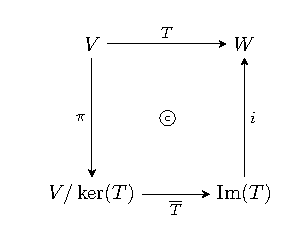
\includegraphics{doc/iso_thm/iso_thm.pdf}
	\caption{Map diagram of the map $\overline{T}$.}
\end{figure}

\begin{proof}
	\textbf{1) $\overline{T}$ is well defined:}. Suppose $x = [v] = [v'] \in V/\ker(T)$, we need to show that $T(v) = T(v')$. Indeed, $[v] = [v']$ implies that $v - v' \in \ker(T)$. Therefore, $T(v - v') = 0$. Since $T$ is linear we conclude that $T(v) = T(v')$.
	
	\textbf{$\overline{T}$ is linear:} Let $\alpha \in K, [v] \in V/\ker(T)$. By the linearity of $T$, the definition of the operations on the quotient space $V/\ker(T)$ and the definition of $\overline{T}$, we have that
	\[
		\overline{T}(\alpha [v]) = \overline{T}([\alpha v]) = T(\alpha v) = \alpha T(v) = \alpha \overline{T}([v]).
	\]
	Now, let $[v_1], [v_2] \in V/\ker(T)$. Then
	\[
		\overline{T}([v_1] + [v_2]) = \overline{T}([v_1 + v_2]) = T(v_1 + v_2) = T(v_1) + T(v_2) = \overline{T}([v_1]) + \overline{T}([v_2]).
	\]
	
	\textbf{2) $\overline{T}$ is injective:} Let $x \in \ker(\overline{T})$. Write $x$ as $x = [v]$ for some $v \in V$. Then
	\[
		\underbrace{\overline{T}(x)}_{\displaystyle = 0} = T(v).
	\]
	Therefore, $v \in \ker(T)$. Thus, $x = [v] = [0_V] = 0_{V/\ker(T)}$.
	
	\textbf{$\overline{T}$ is surjective:} Let $w \in \operatorname{Im}(T)$. Then there exists a $v \in V$ s.t. $T(v) = w$. Therefore, $\overline{T}([v]) = T(v) = w$. This shows that $\operatorname{Im}(T) \subseteq \operatorname{Im}(\overline{T})$.
	
	But by the definition of $\overline{T}$ we also have that $\operatorname{Im}(\overline{T}) \subseteq \operatorname{Im}(T)$.
	
	\textbf{3) The diagram commutes:} Let $v \in V$ and $w \in \operatorname{Im}(T) \subseteq W$ s.t. $T(v) = w$. Then by the definition of $\pi, \overline{T}$ and $i$, we have that
	\[
		(i \circ \overline{T} \circ \pi)(v) = (i \circ \overline{T})([v]) = i\big(T(v)\big) = i(w) = w.
	\]
	\qedhere
\end{proof}

\subsubsection{Universal Propertiy of Quotient Spaces}

\begin{theorem}{Universal Property of Quotient Spaces}{univ_prop_quot_space}
	Let $V$ be a vector space over $K$ and $U \subseteq V$ a subspace. The quotient space $V/U$ has the following universal property: 
	
	For every space $W$ and every linear map $T:V \to W$, for which $T(U) = 0$(, i.e., for which $U \subseteq \ker(T)$), there exists a \textbf{unique} linear map $T':V/U \to W$ s.t. the diagram in Figure \ref{fig:univ_prop} commutes. Moreover, $\ker(T') = \ker(T)/U$.
\end{theorem}
\begin{figure}[h]
	\centering
	\label{fig:univ_prop}
	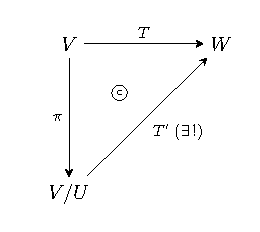
\includegraphics{doc/universal_property/universal_property.pdf}
	\caption{Map diagram of the map $T'$.}
\end{figure}

\textbf{Jargon:} Every linear map $T:V \to W$ that maps $U$ to 0 factors through $V/U$(, i.e., $T = T' \circ \pi$), and moreover in a unique way. We say that $T$ \textbf{induces} a map $T':V/U \to W$. We also say that $T$ \textbf{descends} to a map $T':V/U \to W$.

\subsubsection{Quotient Spaces \& Complements}

\begin{proposition}{A Canonical Isomorphism to a Complement}{canon_iso_compl}
	Let $V$ be a vector space over $K$ and $U \subseteq V$ a subspace. Let $W \subseteq V$ be a complement of $U$. Then there exists a canonical isomorphism $Q:W \overset{\cong}{\longrightarrow} V/U$, defined by
	\[
		Q(w) := [w] \in V/U \qquad \forall w \in W.
	\]
\end{proposition}

\begin{remark}
	The isomorphism $Q$ is canonical, only once $W$ is specified. In general there is no canonical choice of a complement $W$ to $U$. (In general there exist many choices of complements $W$ to $U$, and there is no preferred choice.)
\end{remark}

\subsection{Relations to Dual Spaces}

\begin{proposition}{Perpendicular Subspace}{purp_subsp}
	Let $V$ be a vector space over $K$ and $U \subseteq V$ a subspace. Define
	\[
		U^{\perp} := \bigl\{\ell \in V^* \;|\; \ell |_{U} = 0\bigr\},
	\]
	i.e., all the functionals on $V$ that vanish on $U$. Then:
	\begin{enumerate}
		\item $U^{\perp} \subseteq V^*$ is a linear subspace.
		\item There exists a \textbf{canonical} isomorphism $\big(V/U\big)^* \cong U^{\perp}$. If we assume that $V$ is finite dimensional then there exists a \textbf{canonical} isomorphism $U^* \cong V^*/U^{\perp}$.
	\end{enumerate}
\end{proposition}

\begin{proposition}{}{prop_perp_im}
	Let $T:V \to W$ be a linear map. Then
	\[
		(\operatorname{Im}(T))^{\perp} = \ker(T^*).
	\]
\end{proposition}





	% 
%
% (c) 2025 Autor, ETH Zürich
%
% !TEX root = linalg_I-II_summary.tex
% !TEX encoding = UTF-8
%

\section{Determinants}
Let 
\[
	A = \begin{pmatrix}
		a & b\\
		c & d
	\end{pmatrix} \in M_{2 \times 2}(K).
\]
There is a very simple criterion to check wether $A$ is invertible or not.

\begin{proposition}{Criterion for Invertibility of a $2 \times 2$ Matrix}{crit_inv_2by2_mat}
	$A$ is invertible if and only if $ad - bc \neq 0$. Moreover, if $A$ is invertible, then
	\[
		A^{-1} = \frac{1}{ad - bc}\, \begin{pmatrix}
			d & -b\\
			-c & a
		\end{pmatrix}.
	\]
	The number $ad - bc$ is $\det(A)$.
\end{proposition}

\begin{definition}{N-Linear Function}{nlin_func}
	Let $D:M_{n\times n}(K) \to K$ be a function. We say that $D$ is \textbf{$n$-linear} if for every $1 \leq i \leq n$, $D$ is a linear function of the $i$-th row when the other $(n-1)$ rows are held fixed.
\end{definition}
We can think of $M_{n\times n }(K)$ as $K_{\text{row}}^n \times \hdots \times K_{\text{row}}^n$ and if
\[
	A = \begin{pmatrix}
		\rule[0.5ex]{1em}{0.4pt} & \alpha_1 & \rule[0.5ex]{1em}{0.4pt}\\
		& \vdots & \\
		\rule[0.5ex]{1em}{0.4pt} & \alpha_n & \rule[0.5ex]{1em}{0.4pt}
	\end{pmatrix}
\]
we write $D(A) = D(\alpha_1, \hdots , \alpha_n)$. Saying that $D$ is $n$-linear means that for all $1 \leq i \leq n$, we have that
\begin{enumerate}
	\item \begin{align*}
		D&(\alpha_1, \hdots , \alpha_i + \alpha_i', \hdots , \alpha_n) = D(\alpha_1, \hdots , \alpha_i, \hdots , \alpha_n) + D(\alpha_1, \hdots , \alpha_i', \hdots , \alpha_n) \\
		\forall& \, \alpha_1, \hdots , \alpha_i, \alpha_i', \hdots , \alpha_n \in K^n_{\text{row}}
	\end{align*}
	\item \begin{align*}
		D&(\alpha_1, \hdots , c \cdot \alpha_i, \hdots, \alpha_n) = c \cdot D(\alpha_1, \hdots , \alpha_i, \hdots, \alpha_n) \\
		\forall& \,c \in K, \,\alpha_1, \hdots \alpha_i, \hdots , \alpha_n \in K^n_{\text{row}}
	\end{align*}
\end{enumerate}

\begin{lemma}{Linear Combinations of $n$-linear Functions}{lin_comb_nlin_func}
	Any linear combination of $n$-linear functions is an $n$-linear function again.
\end{lemma}

\begin{definition}{Alternating Functions}{alt_func}
	Let $D:M_{n\times n}(K) \to K$ be an $n$-linear function. We say that $D$ is \textbf{alternating} if for every matrix $A \in M_{n\times n}(K)$ in which some two rows are equal we have that $D(A) = 0$.
\end{definition}

\begin{proposition}{}{prop_alt}
	Let $D$ be an $n$-linear function. Assume that $D$ has the property that whenever $A$ has two equal adjacent (aufeinanderfolgende) rows then $D(A) = 0$. Then
	\begin{enumerate}
		\item $D$ is alternating.
		\item For every matrix $B$, if $B'$ is obtained from $B$ by interchanging any two of its rows, then $D(B') = -D(B)$.
	\end{enumerate}
\end{proposition}

\begin{definition}{Determinant Function}{det_func}
	A function $D:M_{n\times n}(K) \to K$ is called \textbf{determinant function} if $D$ is $n$-linear, is alternating and $D(I) = 1$.
\end{definition}

\begin{definition}{Row\&Column-Deletion Matrix}{row_col_del_mat}
	Let $A \in M_{n\times n}(K)$, $n \geq 2$, $1 \leq i \leq n$, $1 \leq j \leq n$. We denote by 
	\[
		A(i|j) \in M_{(n-1)\times (n-1)}(K)
	\]
	the matrix obtained from $A$ by deleting row \#$i$ and column \#$j$.
	
	If $D$ is an $(n-1)$-linear function and $A \in M_{n\times n}(K)$ we denote
	\[
		D_{ij}(A) := D\big(A(i|j)\big).
	\]
\end{definition}

\textbf{Notation:} Let $A \in M_{m\times n}(K)$ and $1 \leq i \leq m$, $1 \leq j \leq n$. Denote the element at position $(i,j)$ in the matrix $A$ by $A(i,j)$ or $A_{ij}$.

\begin{theorem}{Entwicklungssatz}{entw_satz}
	Let $n \geq 2$ and $D$ an $(n-1)$-linear function, which is alternating. Let $1 \leq j \leq n$. Define a function $E_j:M_{n\times n}(K) \to K$ by
	\[
		E_j(A) := \sum_{i=1}^{n} (-1)^{i+j} A_{ij} \, D_{ij}(A).
	\]
	Then $E_j$ is an $n$-linear function and is alternating. If $D$ is a determinant function then so is $E_j$.
\end{theorem}

\begin{corollary}{Existence of a Determinant Function}{exist_det_func}
	$\forall \, n \geq 1$, there exists at least one determinant function $M_{n\times n}(K) \to K$.
\end{corollary}

\subsection{Uniqueness of the Determinant}
Let $D:M_{n\times n}(K) \to K$ be an $n$-linear alternating function. Let
\[
	A = \begin{pmatrix}
		\rule[0.5ex]{1em}{0.4pt} & \alpha_1 & \rule[0.5ex]{1em}{0.4pt}\\
		& \vdots & \\
		\rule[0.5ex]{1em}{0.4pt} & \alpha_n & \rule[0.5ex]{1em}{0.4pt}
	\end{pmatrix} \in M_{n\times n}(K).
\]
Denote
\[
	I = \begin{pmatrix}
		1 & \hdots & 0\\
		\vdots &\ddots & \vdots\\
		0 & \hdots & 1
	\end{pmatrix}
	=
	\begin{pmatrix}
		\rule[0.5ex]{1em}{0.4pt} & \varepsilon_1 & \rule[0.5ex]{1em}{0.4pt}\\
		& \vdots & \\
		\rule[0.5ex]{1em}{0.4pt} & \varepsilon_n & \rule[0.5ex]{1em}{0.4pt}
	\end{pmatrix}.
\]
(So, $\varepsilon_1, \hdots , \varepsilon_n$ is the standard basis of $K^n_{\text{row}}$.) Clearly, 
\[
	\alpha_i = \sum_{j=1}^{n} A(i,j)\, \varepsilon_j \qquad \forall \, 1\leq i \leq n.
\]
Therefore,
\begin{align*}
	D(A) &= D(\alpha_1, \hdots , \alpha_n) = D\bigg( \sum_{j=1}^{n} A(1,j) \, \varepsilon_j, \alpha_2, \hdots , \alpha_n\bigg) = \sum_{j=1}^{n} A(1,j) \cdot D(\varepsilon_j, \alpha_2, \hdots , \alpha_n) \\
	&= \sum_{j=1}^{n} A(1, j)\cdot D\bigg(\varepsilon_j, \sum_{k=1}^{n} A(2, k)\, \varepsilon_k, \hdots, \alpha_n\bigg) = \sum_{j,k = 1}^{n} A(1,j)\cdot A(2,k) \cdot D(\varepsilon_j, \varepsilon_k, \hdots, \alpha_n).
\end{align*}
Applying these steps to every row we get that
\begin{equation}
	\label{eq:det_func}
	D(A) = \sum_{k_1, \hdots, k_n = 1}^{n} A(1, k_1)\cdot A(2, k_2)\cdot \hdots \cdot A(n, k_n)\cdot D(\varepsilon_{k_1}, \varepsilon_{k_2} \hdots, \varepsilon_{k_n}),
\end{equation}
where each of the indices $k_1, \hdots , k_n$ runs between $1$ and $n$. So far we haven't used the fact that $D$ is alternating. Now, since $D$ is alternating $D(\varepsilon_{k_1}, \hdots , \varepsilon_{k_n}) = 0$, whenever two of the indices $k_1, \hdots , k_n$ are equal. So, we are interested only in ordered sequences of indices $(k_1, \hdots, k_n)$ in which $k_i \in \{1, \hdots, n\} \quad \forall i$ and $k_i \neq k_j \quad \forall i \neq j$. Such a sequence is called a permutation of $\{1, \hdots , n\}$, or a permutation of degree $n$.

\begin{definition}{Permutation}{permut}
	A \textbf{permutation} is a bijective map $\sigma :\{1, \hdots, n\} \to \{1, \hdots, n\}$.
\end{definition}

So Alternatively, we can think of a permutation of degree $n$ as a bijective function $\sigma:\{1,\hdots , n\} \to \{1, \hdots , n\}$. Then the sequence $(k_1, \hdots, k_n) = (\sigma 1, \hdots, \sigma 2)$ is a permutation as defined earlier. (Notation: $\sigma(i) := \sigma i$.). In other words, a permutation $\sigma$ of degree $n$ is a re-ordering of a list with $n$ elements $(1,\hdots, n) \overset{\sigma}{\longrightarrow} (\sigma 1, \hdots, \sigma n)$.

We can rewrite Equation \eqref{eq:det_func} as
\[
	D(A) = \sum_{\sigma \in S_n} A(1, \sigma 1)\cdot \hdots \cdot A(n, \sigma n) \cdot D(\varepsilon_{\sigma 1}, \hdots , \varepsilon_{\sigma n}),
\]
where $S_n$ is the set of all permutations of degree $n$.

\subsubsection{Important Thing About Permutations}
Let $\sigma$ be a permutation of degree $n$. Then one can pass from $(1, \hdots , n)$ to $(\sigma 1, \hdots , \sigma n)$ by performing a finite sequence of interchanges of pairs, called transpositions.

\begin{definition}{Transposition}{transposition}
	A \textbf{transposition} is a permutation $\theta :\{1, \hdots, n\} \to \{1, \hdots, n\}$, where $\exists \, i,j \in \{1, \hdots, n\}$, $i \neq j$ s.t. $\theta(i) = j$,  $\theta(j) = i$ and $\theta(k) = k \quad \forall \, k\neq i,j$.
\end{definition}

Now, every permutation $\sigma :\{1, \hdots, n\} \to \{1, \hdots, n\}$ can be written as a composition of transpositions
\begin{equation}
	\label{eq:permut_transp}
	\sigma = \theta_1 \circ \hdots \circ \theta_m,
\end{equation}
where $\theta_1, \hdots, \theta_m$ are transpositions. But these $\theta_i$'s and $m$ are not unique. In other words, the same $\sigma$ can be written as in Equation \eqref{eq:permut_transp} in many different ways
\[
	\sigma = \theta_1 \circ \hdots \circ \theta_m = \theta_1' \circ \hdots \circ \theta_{m'}'.
\]
Why Can $\sigma$ be written as in \eqref{eq:permut_transp}. Start with $(1, \hdots , n)$ and if $\sigma 1 \neq 1$ then interchange $1$ and $\sigma 1$. We now have $(\sigma 1, \hdots , 1, \hdots , n)$. If $\sigma 2 \neq 2$, then interchange $1 $ and $\sigma 2$; otherwise proceed to $3$, etc. But of course there are other ways to do it, e.g., $(3, 2, 1)$ can be obtained in 3 steps: $(1,2,3) \to (2,1,3) \to (2,3,1) \to (3,2,1)$. But also in one step $(1,2,3) \to (3,2,1)$.

\begin{definition}{\textcolor{red}{Sign of a Permutation}}{sgn_permut}
	Let $\sigma$ be a permutation and let $\theta_1, \hdots, \theta_m$ be transpositions s.t. $\sigma = \theta_1 \circ \hdots \circ \theta_m$. The permutation $\sigma$ is called \textbf{even} if $m$ is even, and is called \textbf{odd} if $m$ is odd. The number $(-1)^m \in \{-1, 1\}$ is called the \textbf{sign} of $\sigma$, i.e., $\operatorname{sgn}(\sigma) := (-1)^m$.
\end{definition}

\begin{lemma}{\textcolor{red}{Well Definedness of the Sign of a Permutation}}{parity_permut}
	If $(\sigma 1, \hdots , \sigma n)$ is obtained from $(1, \hdots , n)$ in two different ways, one time by a sequence of $m$ transpositions, and another time by a sequence of $m'$ transpositions, then $m'$ and $m$ have the same parity, i.e., $(-1)^{m'} = (-1)^m$.
	
	(So the parity of $m$ depends only on $\sigma$ and not on the particular way we performed a sequence of transpositions $(1, \hdots , n) \to \hdots \to (\sigma 1, \hdots, \sigma n)$.)
\end{lemma}

\begin{proof}
	We know that determinant functions $M_{n\times n}(K) \to K$ exists for every $n \geq 1$. Fix a determinant function $E:M_{n\times n}(K) \to K$. Consider $E(\varepsilon_{\sigma 1}, \hdots , \varepsilon_{\sigma n})$. If $(\sigma 1, \hdots, \sigma n)$ can be obtained from $(1, \hdots, n)$ by a sequence of $m$ transpositions, then the matrix
	\[
		\begin{pmatrix}
			\rule[0.5ex]{1em}{0.4pt} & \varepsilon_1 & \rule[0.5ex]{1em}{0.4pt}\\
			& \vdots & \\
			\rule[0.5ex]{1em}{0.4pt} & \varepsilon_n & \rule[0.5ex]{1em}{0.4pt}
		\end{pmatrix}
	\]
	can be obtained from
	\[
		I = \begin{pmatrix}
			1 & \hdots & 0\\
			\vdots &\ddots & \vdots\\
			0 & \hdots & 1
		\end{pmatrix}
	\]
	by a sequence of $m$ interchanges of pairs of rows. Therefore,
	\[
		E(\varepsilon_{\sigma 1}, \hdots, \varepsilon_{\sigma n}) = (-1)^m E(\varepsilon_1, \hdots, \varepsilon_n) = (-1)^m E(I) = (-1)^m.
	\]
	But this applies also to $m'$. So, 
	\[
		E(\varepsilon_{\sigma 1}, \hdots, \varepsilon_{\sigma n}) = (-1)^{m'}E(\varepsilon_1, \hdots, \varepsilon_n) = (-1)^{m'} E(I) = (-1)^{m'}.
	\]
	So we have that
	\[
		(-1)^m = (-1)^{m'}.
	\]
	\qedhere
\end{proof}

\subsubsection{Back to our $D(A)$}
We have seen that if $D$ is $n$-linear and alternating then
\[
	D(A) = \sum_{\sigma \in S_n} A(1, \sigma 1)\cdot \hdots \cdot A(n, \sigma n) \cdot D(\varepsilon_{\sigma 1}, \hdots , \varepsilon_{\sigma n}).
\]
But 
\begin{equation}
	\label{eq:det_permut}
	D(\varepsilon_{\sigma 1}, \varepsilon_{\sigma n}) = (\operatorname{sgn}\sigma)\cdot D(\varepsilon_1, \hdots, \varepsilon_n) = (\operatorname{sgn}\sigma)\cdot D(I)
\end{equation}

\begin{theorem}{Uniqueness of the Determinant Function}{unique_det_func}
	$\forall \, n \geq 1$, there exists a unique determinant function $M_{n\times n}(K) \to K$. We will denote it by $\det$. It is given by the formula
	\[
		\det(A) = \sum_{\sigma \in S_n} A(1, \sigma 1)\cdot \hdots \cdot A(n, \sigma n).
	\]
\end{theorem}

\begin{corollary}{}{cor_nlin_alt_func}
	For every $n$-linear and alternating function $D:M_{n\times n}(K) \to K$ we have that
	\[
		D(A) = \det(A)\cdot D(I) \qquad \forall \, A \in M_{n\times n}(K).
	\]
\end{corollary}

\subsubsection{A Bit more on Permutations}
Denote by $S_n$ the set of permutations $\sigma :\{1, \hdots, n\} \to \{1, \hdots, n\}$. $S_n$ has the structure of a group:
\begin{itemize}
	\item[$\bullet$] We can compose permutations, i.e., if $\sigma, \tau :\{1, \hdots, n\} \to \{1, \hdots, n\}$, then $\sigma \cdot \tau := \sigma \circ \tau$, where $\sigma \circ \tau :\{1, \hdots, n\} \to \{1, \hdots, n\}$.
	\item[$\bullet$] The identity $id :\{1, \hdots, n\} \to \{1, \hdots, n\}$ is the neutral element $1 \in S_n$. 
	\item[$\bullet$] The inverse $\sigma^{-1}$ of $\sigma$, is given by the inverse of the function $\sigma$ (recall that $\sigma$ is bijective, so $\sigma^{-1}$ does exist).
\end{itemize}
Also, note that $|S_n| = n!$

\begin{lemma}{Sign of the Composition of Permutations}{sgn_comp_permut}
	$\forall \, \sigma, \tau \in S_n$ we have 
	\[
		\operatorname{sgn}(\sigma \cdot \tau) = \operatorname{sgn}(\sigma)\cdot \operatorname{sgn}(\tau).
	\]
\end{lemma}

\begin{theorem}{\textcolor{red}{The Determinant of the Product of Two Matrices}}{det_prod_mat}
	$\forall \, A,B \in M_{n\times n}(K)$ we have that
	\[
		\det(A\cdot B) = \det(A) \cdot \det(B).
	\]
\end{theorem}

\begin{proof}
	Fix a matrix $B \in M_{n\times n}(K)$, and consider a function $D:M_{n\times n}(K) \to K$ defined by
	\[
		D(A) := \det(A\cdot B).
	\]
	
	\textbf{Claim:} $D$ is $n$-linear and alternating.
	
	\textbf{Proof of Claim:} Write
	\[
		A = \begin{pmatrix}
			\rule[0.5ex]{1em}{0.4pt} & \alpha_1 & \rule[0.5ex]{1em}{0.4pt}\\
			& \vdots & \\
			\rule[0.5ex]{1em}{0.4pt} & \alpha_n & \rule[0.5ex]{1em}{0.4pt}
		\end{pmatrix}.
	\]
	If we view $\alpha_i$ as a $1 \times n$ matrix, then $\alpha_i B$ is also $1 \times n$, and in fact
	\[
		A\cdot B = \begin{pmatrix}
			\rule[0.5ex]{1em}{0.4pt} & \alpha_1 B & \rule[0.5ex]{1em}{0.4pt}\\
			& \vdots & \\
			\rule[0.5ex]{1em}{0.4pt} & \alpha_n B & \rule[0.5ex]{1em}{0.4pt}
		\end{pmatrix}.
	\]
	So, 
	\[
		D(A) = \det(\alpha_1 B, \hdots, \alpha_n B).
	\]
	Clearly, for every two row vectors $\alpha_i, \alpha_i'$ we have that $(\alpha_i + \alpha_i') B = \alpha_i B + \alpha_i' B$ and
	\[
		\forall \, c\in K : \; (c \cdot \alpha_i) B = c \cdot (\alpha_i B).
	\]
	Since $\det$ is $n$-linear it follows that $D$ is also $n$-linear.
	
	If $\alpha_i = \alpha_j$, then $\alpha_i B = \alpha_j B$. Therefore, 
	\[
		D(A) = \det(\alpha_1 B, \hdots, \alpha_n B) = 0.
	\]
	This proves the claim.
	
	We continue with the proof of the Theorem. Since we found that $D$ is $n$-inear and alternating, by Corollary \ref{cor*cor_nlin_alt_func}, we have that
	\[
		D(A) = \det(A)\cdot D(I).
	\]
	But $D(I) = \det(I\cdot B) = \det(B)$. Therefore, 
	\[
		D(A) = \det(A \cdot B) = \det(A)\cdot \det(B). \qedhere
	\]
\end{proof}

\begin{corollary}{Equivalent Condition for The Invertibility of a Matrix}{equiv_cond_inv_mat}
	If $A$ is invertible then $\det(A) \neq 0$. Moreover,
	\[
		\det(A^{-1}) = \frac{1}{\det(A)}.
	\]
\end{corollary}

\subsection{More on Determinants}

\begin{theorem}{Determinant of a Transposed Matrix}{det_trans_mat}
	$\forall \, A \in M_{n\times n}(K) : \; \det(A^T) = \det(A)$.
\end{theorem}

\begin{corollary}{}{cor_alt_func_2}
	If $D:M_{n\times n}(K) \to K$ is an alternating $n$-linear function (of the rows of a matrix) then $D$ is also an alternating and $n$-linear function of the columns of a matrix. In fact, $D(A^T) = D(A) \quad \forall \, A\in M_{n\times n}(K)$. In particular, this holds also for $D = \det$.
\end{corollary}

\begin{theorem}{Determinant after Row/Column Operations}{det_row_op}
	\begin{enumerate}
		\item If $B$ is obtained from $A$ by adding a multiple of one row of $A$ to another row (or by doing the analogous operation on columns), then $\det(B) = \det(A)$.
		\item If $A \overset{R_i \leftrightarrow R_j}{\longrightarrow} B$, $i \neq j$, (or the analogous operation on columns) then $\det(B) = -\det(A)$.
		\item If $A \overset{c\cdot R_i \to R_i}{\longrightarrow} B$, then $\det(B) = c \cdot \det(A)$.
	\end{enumerate}
\end{theorem}

\subsubsection{Determinants of Block Matrices}
Consider a block matrix $M$ of the type
\[
	M = \begin{pmatrix}
		A & B\\
		0 & C
	\end{pmatrix},
\]
where $A \in M_{r\times r}(K)$, $C \in M_{s \times s}(K)$, $B \in M_{r \times s}(K)$.

\begin{proposition}{Determinant of a Block Matrix}{det_block_mat}
	Let $M$ be as above. Then
	\[
		\det(M) = \det(A) \cdot \det(C).
	\]
\end{proposition}

\begin{corollary}{Entwicklungssatz with Cofactors}{entwick_satz_cofact}
	$\forall \, A \in M_{n\times n}(K)$ we have the following $n$ different formulas for $\det(A)$, i.e.,
	\[
		\det(A) = \sum_{i=1}^{n} (-1)^{i+j} A_{ij} \det\big(A(i|j)\big), \quad j = 1, \hdots, n.
	\]
	The scalars $c_{ij} := (-1)^{i+j} \det\big(A(i|j)\big)$ are called the $i, j$ \textbf{cofactor} of $A$. We have
	\begin{equation}
		\label{eq:det_cofactor}
		\det(A) = \sum_{i=1}^{n} A_{ij}\cdot c_{ij}.
	\end{equation}
\end{corollary}

\textbf{Claim:} If we replace $A_{ij}$ in Equation \eqref{eq:det_cofactor} by $A_{ik}$, where $k$ is fixed, we always get 0. In other words, $\forall \, A \in M_{n\times n}(K)$, $\forall \, j$ we have
\[
	\sum_{i=1}^{n} A_{ik} \cdot c_{ij} = \begin{cases}
		\det(A) & j = k\\
		0 & j \neq k
	\end{cases}.
\]

\textbf{Proof of Claim:} Let $B \in M_{n \times n}(K)$ be the matrix obtained from $A$ by replacing column $j$ of $A$ by column $k$ of $A$. So, in $B$ column $j$ equals column $k$. Clearly, $\det(B) = 0$ since $B$ has two equal columns ($\Longleftrightarrow \; B^T$ has two equal rows). 
\[
	\Longrightarrow \qquad 0 = \det(B) = \sum_{i=1}^{n} (-1)^{i+j} B_{ij} \det\big(B(i|j)\big)= \sum_{i=1}^{n}  = \sum_{i=1}^{n} A_{ik} \det\big(A(i|j)\big) = \sum_{i=1}^{n} A_{ik} \cdot c_{ij}.
\]
This proves the claim.

So, $\forall \, A \in M_{n\times n}(K)$, $\forall \, j,k$ we have 
\begin{equation}
	\label{eq:det_cofactor_2}
	\sum_{i=1}^{n} A_{ik} \cdot c_{ij} = \delta_{jk} \cdot \det(A).
\end{equation}

\begin{definition}{Classical Adjoint of $A$}{classic_adjoint}
	The matrix $(c_{ij})^T$ is called the \textbf{classical adjoint of $A$}, i.e.,
	\[
		\operatorname{adj}(A) \in M_{n \times n}(K), \qquad \big(\operatorname{adj}(A)\big)_{ij} = c_{ji} = (-1)^{i+j} \cdot \det\big(A(j|i)\big).
	\]
\end{definition}

The Equation \eqref{eq:det_cofactor_2} says that
\[
	\label{eq:adjoint}
	(\operatorname{adj}A) \cdot A = \det(A) \cdot I.
\]
Indeed, 
\begin{align*}
	 \det(A) \cdot \delta_{jk} &= \sum_{i=1}^{n} c_{ij} \cdot A_{ik} = \sum_{i=1}^{n} \big(\operatorname{adj}(A)\big)_{ji} \cdot A_{ik} \\
	 \Longrightarrow \qquad \det(A) \cdot I &= \operatorname{adj}(A) \cdot A.
\end{align*}

\begin{theorem}{Formula for the inverse of $A$}{formula_inv}
	Let $A \in M_{n\times n}(K)$. Then $A$ is invertible if and only if $\det(A) \neq 0$. When $A$ is invertible we have
	\[
		A^{-1} = \frac{1}{\det(A)} \, \operatorname{adj}(A).
	\]
\end{theorem}

\subsection{Cramer's Rule}
Let $A \in M_{n\times n}(K)$. We would like a formula to solve the system of equations $A x = b$, where
\[
	x = \begin{pmatrix}
		x_1\\
		\vdots \\
		x_n
	\end{pmatrix}
\]
are the unknowns and
\[
	b= \begin{pmatrix}
		b_1\\
		\vdots \\
		b_n
	\end{pmatrix} \in K^n
\]
is given. Assume $Ax = b$. Then
\begin{align*}
	\operatorname{adj}A \cdot A x &= \operatorname{adj}A \cdot b\\
	\Longrightarrow \qquad \det(A) \cdot x &= \operatorname{adj}\cdot b\\
	\Longrightarrow \qquad \forall \, 1 \leq j \leq n : \; \det(A)\cdot x_j &= \sum_{i=1}^{n} (\operatorname{adj}A)_{ji}\cdot  b_i = \sum_{i=1}^{n} (-1)^{i+j} b_i \det\big(A(i|j)\big),
\end{align*}
where the last expression is the determinant of the matrix obtained from $A$ by replecing column $j$ by $b$.

\begin{theorem}{Cramer's Rule}{cramers_rule}
	Let $A \in M_{n\times n}(K)$ with $\det(A) \neq 0$. Let $b \in K^n$. Then the system $A x = b$ has a unique solution, and it is given by the formula
	\[
		x_j = \frac{\det\big(A(j, b)\big)}{\det(A)} \qquad \forall \, 1 \leq j \leq n,
	\]
	where $A(j, b)$ is the matrix obtained from $A$ by replacing column $j$ by $b$.
\end{theorem}

\subsection{Determinants of Endomorphisms}
Let $A \in M_{n \times n}(K)$ and $P \in GL_n(K)$, then 
\[
	\det(P^{-1} A P) = \det(P^{-1}) \cdot \det(A) \cdot \det(P) = \frac{1}{\det(P)}\cdot \det(A) \cdot \det(P) = \det(A).
\]
In other words, similar matrices have the same determinant.

Let $V$ be a finite dimensional vector space over $K$. Put $n := \dim V$. Let $T:V \to V$ be a linear map. Pick a basis $\mathcal{B}$ for $V$. We have a matrix $[T]^{\mathcal{B}}_{\mathcal{B}} \in M_{n\times n}(K)$. Consider $\det [T]^{\mathcal{B}}_{\mathcal{B}} \in K$.

\textbf{Question:} Does $\det [T]^{\mathcal{B}}_{\mathcal{B}}$ depend on the basis $\mathcal{B}$?

\textbf{Answer:} Let $\mathcal{B}'$ be another basis for $V$. Denote by $P := [id_V]^{\mathcal{B}'}_{\mathcal{B}}$ the transition matrix between the basis $\mathcal{B}'$ and $\mathcal{B}$. Recall that
\[
	[T]^{\mathcal{B}'}_{\mathcal{B}} = [id_V]^{\mathcal{B}}_{\mathcal{B}'} \cdot [T]^{\mathcal{B}}_{\mathcal{B}} \cdot [id_V]^{\mathcal{B}'}_{\mathcal{B}},
\]
and we also have $[id_V]^{\mathcal{B}}_{\mathcal{B}'} = \big([id_V]^{\mathcal{B}'}_{\mathcal{B}}\big)^{-1}$. So, 
\[
	[T]^{\mathcal{B}'}_{\mathcal{B}'} = P^{-1} \cdot [T]^{\mathcal{B}}_{\mathcal{B}} \cdot P. \qquad \Longrightarrow \qquad \det [T]^{\mathcal{B}'}_{\mathcal{B}'} = \det [T]^{\mathcal{B}}_{\mathcal{B}}.
\]
Recall also that if $T, S:V \to V$ are two linear maps then $[S \circ T]^{\mathcal{B}}_{\mathcal{B}} = [S]^{\mathcal{B}}_{\mathcal{B}} \cdot [T]^{\mathcal{B}}_{\mathcal{B}}$. Recall also that if $T:V \to V$ is an isomorphism then $[T^{-1}]^{\mathcal{B}}_{\mathcal{B}} = \big([T]^{\mathcal{B}}_{\mathcal{B}}\big)^{-1}$. Finally, $[id_V]^{\mathcal{B}}_{\mathcal{B}} = I$.

\begin{corollary}{\textcolor{red}{Well Definedness of the Determinant of an Endomorphism}}{det_endo_well_def}
	Let $V$ be a finite dimensional vector space over $K$. Let $T:V \to V$ be a linear map. Then $\det [T]^{\mathcal{B}}_{\mathcal{B}}$ does \textbf{not} depend on the choice of basis $\mathcal{B}$ of $V$. We denote this scalar by $\det(T) \in K$. The function
	\[
		\det: \operatorname{End}(V) \to K, \quad T \mapsto \det(T)
	\]
	has the following properties:
	\begin{enumerate}
		\item $\det(S \circ T) = \det(S) \cdot \det(T) \qquad \forall \, S, T \in \operatorname{End}(V)$.
		\item $T$ is an isomorphism if and only if $\det(T) \neq 0$. If $T$ is an isomorphism then 
		\[
			\det(T^{-1}) = \frac{1}{\det(T)}.
		\]
		\item $\det(id_V) = 1$.
		\item $\det(0) = 0 \in K$.
	\end{enumerate}
\end{corollary}

\begin{remark}
	In contrast to $T:V \to V$, if we take $T:V \to W$, and $\mathcal{B}, \mathcal{C}$ bases of $V, W$, then $\det [T]^{\mathcal{B}}_{\mathcal{C}}$ \textbf{depends} on $\mathcal{B}, \mathcal{C}$ (unless $W = V$ and $\mathcal{C} = \mathcal{B}$).
\end{remark}
	% 
%
% (c) 2025 Autor, ETH Zürich
%
% !TEX root = linalg_I-II_summary.tex
% !TEX encoding = UTF-8
%

\section{Eigenvalues \& Eigenvectors}
\begin{definition}{Eigenvalues \& Eigenvectors}{eigval_eigvect}
	Let $V$ be a vector space over $K$ and $T:V \to V$ a linear map (an endomorphism of $V$). We say that $\lambda \in K$ is an \textbf{eigenvalue} of $T$ if $\exists\, v \in V \setminus \{0\}$ s.t. 
	\[
		Tv = \lambda v.
	\]
	Any vector $v \in V\setminus \{0\}$ with the property that $Tv = \lambda v$ is called an \textbf{eigenvector} of $T$ for the eigenvalue $\lambda$.
\end{definition}

\begin{definition}{Diagonalizability}{diagon}
	Let $V$ be a finite dimensional vector space over $K$ and $T:V \to V$ a linear map. We say that $T$ is diagonalizable if there exists a basis $\mathcal{B}$ of $V$ s.t.
	\begin{equation}
		\label{eq:diagon_mat}
		[T]^{\mathcal{B}}_{\mathcal{B}} = \begin{pmatrix}
			\lambda_1 & \hdots & 0\\
			\vdots & \ddots & \vdots\\
			0 & \hdots & \lambda_n
		\end{pmatrix}.
	\end{equation}
\end{definition}

\begin{lemma}{Equivalent Condition for Diagonalizability}{equiv_cond_diagon}
	$T$ is diagonalizable if and only if there exists a basis $\mathcal{B} = (v_1, \hdots , v_n)$ consisting of eigenvectors of $T$ (i.e., $\forall \, i, \; Tv_i = \lambda_i v_i$ for some $\lambda_i \in K$). Moreover, if for some basis $\mathcal{B} = (v_1, \hdots , v_n)$ the matrix $[T]^{\mathcal{B}}_{\mathcal{B}}$ has the shape as in Equation \eqref{eq:diagon_mat}, then $\forall \, i$, $\lambda_i$ is an eigenvalue of $T$ and $v_i$ is an eigenvector of $\lambda_i$.
\end{lemma}

\begin{remark}
	We saw that $\forall \, A\in M_{n\times n}(K)$ we have a linear map $T_A:K^n \to K^n, \; T_A(v) := Av$. We say that $A \in M_{n\times n}(K)$ is diagonalizable if the linear map $T_A$ is diagonalizable.
\end{remark}

\begin{proposition}{\textcolor{red}{Linear Independence of Eigenvectors of Distinct Eigenvalues}}{lin_indep_dist_eigenvect}
	Let $V$ be a vector space over $K$ and $T:V \to V$ a linear map. Suppose that $\lambda_1, \hdots , \lambda_n \in K$ are eigenvalues of $T$ which are pairwise distinct (i.e., $\lambda_i \neq \lambda_j \quad \forall \, i \neq j$). Let $v_1, \hdots , v_n$ be eigenvectors for $\lambda_1, \hdots, \lambda_n$ respectively. Then $v_1, \hdots, v_n$ are linearly independent.
\end{proposition}

\begin{proof}
	Induction on $n$.
	
	\textbf{$n = 1$:} $v_1$ is an eigenvector for $\lambda_1$. By definition of $v_1 \neq 0$. $\Longrightarrow \; v_1$ is linearly independent.
	
	\textbf{Induction step:} Let $n \geq 1$ and suppose the proposition holds for any list of $n$ eigenvalues and eigenvectors. We'll prove now that the propostion holds also fro a list of $n+1$ eigenvalues and eigenvectors. Let $\lambda_1, \hdots, \lambda_n, \lambda_{n+1}$ be pairwise distinct eigenvalues of $T$, and $v_1, \hdots , v_n, v_{n+1}$ a given list of eigenvectors of $\lambda_1, \hdots, \lambda_n, \lambda_{n+1}$, respectively. We need to prove that $v_1, \hdots , v_n, v_{n+1}$ are linearly independent.
	
	Assume that 
	\begin{equation}
		\label{eq:distinct_eigenval_1}
		a_1v_1 + \hdots + a_n v_n + a_{n+1} v_{n+1} = 0.
	\end{equation}
	We need to show that $a_1 = \hdots = a_n = a_{n+1} = 0$. Apply $T$ to Equation \eqref{eq:distinct_eigenval_1}. Since $T$ is linear, we have that
	\[
		a_1 Tv_1 + \hdots + a_n Tv_n + a_{n+1} Tv_{n+1} = 0.
	\]
	But $\forall \,i :\; Tv_i = \lambda_i v_i$. Therefore,
	\begin{equation}
		\label{eq:distinct_eigenval_2}
		a_1 \lambda_1 v_1 + \hdots, a_n \lambda_n v_n + a_{n+1}\lambda_{n+1}v_{n+1} = 0.
	\end{equation}
	Consider now Equation \eqref{eq:distinct_eigenval_2} - $\lambda_{n+1} \cdot $\eqref{eq:distinct_eigenval_1}, i.e.,
	\[
		a_1 (\lambda_1 - \lambda_{n+1}) v_1 + \hdots + a_n (\lambda_n - \lambda_{n+1}) v_n + a_{n+1}\underbrace{(\lambda_{n+1} - \lambda_{n+1})}_{\displaystyle = 0}v_{n+1} = 0.
	\]
	By the induction hypothesis $v_1, \hdots , v_n$ are linearly independent. Therefore,
	\[
		a_1 (\lambda_1 - \lambda_{n+1}) =  \hdots = a_n (\lambda_n - \lambda_{n+1}) = 0.		
	\]
	By assumption $\lambda_i \neq \lambda_{n+1} \quad \forall\, 1 \leq i \leq n$. So we have that $a_1 = \hdots = a_n = 0$. Going back to Equation \eqref{eq:distinct_eigenval_1} we get that $a_{n+1} \cdot v_{n+1} = 0$. But by assumption we also have that $v_{n+1} \neq 0$. Therefore, $a_{n+1} = 0$. \qedhere
\end{proof}

\subsection{The Characteristic Polynomial}
\begin{proposition}{Equivalent Condition for Eigenvalue}{equiv_cond_eigenval}
	Let $V$ be a vector space over $K$ and $T:V \to V$ a linear map. Then $\lambda \in K$ is an eigenvalue of $T$ if and only if the linear map $T - \lambda \cdot id$ is \textbf{not} injective.
\end{proposition}

\begin{definition}{The Characterstic Polynomial}{char_poly}
	Let $V$ be a finite dimensional vector space over $K$ and $T:V \to V$ a linear map. We define the \textbf{characteristic polynomial of $T$} as
	\[
		p_T(x) := \det(T - x \cdot id_V).
	\]
	We define the characteristic polynomial of a matrix $A \in M_{n\times n}(K)$ in the same way, i.e.,
	\[
		p_A(x) := \det(A - x \cdot I_n).
	\]
\end{definition}

\begin{definition}{Eigenspace}{eigenspace}
	Let $V$ be a vector space over $K$ and $T \in \operatorname{End}(V)$. Let $\lambda \in K$ be an eigenvalue of $T$. The \textbf{eigenspace} corresponding to $\lambda$ is defined as
	\begin{align*}
		\operatorname{Eig}_T(\lambda) := \{ v \in V \;|\; Tv = \lambda v\} = \ker(T - \lambda id_V) = \{v \in V \;|\: v \text{ is an eigenvector of } \lambda\} \cup \{0\}.
	\end{align*}
	Clearly, since $\operatorname{Eig}_T(\lambda)$ is the kernel of a linear map, $\operatorname{Eig}_T(\lambda) \subseteq V$ is a linear subspace of $V$.
\end{definition}

\begin{lemma}{Properties of the Characteristic Polynomial}{prop_char_poly}
	Let $A \in M_{n\times n}(K)$. Then:
	\begin{enumerate}
		\item $p_A(x)$ is a polynomial of degree $n$, with leading coefficient $(-1)^n$, i.e., $p_A(x) = c_n x^n + c_{n-1}x^{n-1} + \hdots + c_1 x + c_0$, with $c_i \in K \quad \forall \, i$, and $c_n = (-1)^n$.
		\item $p_{A^T}(x) = p_A(x)$.
		\item If $A$ has upper triangular form as in Definition \ref{def*triang_diag_mat}, then
		\[
			p_A(x) = (\lambda_1 - x)\cdot \hdots \cdot (\lambda_n - x).
		\]
		\item If
		\[
			A = \begin{pmatrix}
				B_1 & \ast\\
				0 & B_2
			\end{pmatrix}
		\]
		is a block matrix, then
		\[
			p_A(x) = p_{B_1}(x) \cdot p_{B_2}(x).
		\]
		\item If $A$ and $B$ are similar matrices, i.e., $B = P^{-1} A P$ for some $P \in GL_n(K)$, then
		\[
			p_A(x) = p_B(x).
		\]
	\end{enumerate}
\end{lemma}

\begin{remark}
	If $V$ is an $n$-dimensional vector space over $K$ and $T \in \operatorname{End}(V)$, then $p_T(x)$ is a polynomial of degree $n$ with leading coefficient $(-1)^n$.
\end{remark}

\begin{definition}{\textcolor{red}{The Trace}}{trace}
	Let $A \in M_{n\times n}(K)$. Define the \textbf{trace} (Spur) of $A$ as
	\[
		\operatorname{Tr}(A) := \sum_{i=1}^{n} A_{ii} \in K,
	\]
	i.e., the sum of the entries along the diagonal of $A$. If $V$ is a finite dimensional vector space over $K$ and $T \in \operatorname{End}(V)$, we define the trace of $T$ as
	\[
		\operatorname{Tr}(T) := \operatorname{Tr}\big([T]^{\mathcal{B}}_{\mathcal{B}}\big),
	\]
	where $\mathcal{B}$ is some basis for $V$. We'll see soon that $\operatorname{Tr}(T)$ is well defined, i.e., it does not depend on the choice of $\mathcal{B}$.
\end{definition}

\begin{lemma}{\textcolor{red}{Properties of the Trace}}{prop_trace}
	\begin{enumerate}
		\item 
		\[
			\forall \, A,B \in M_{n\times n}(K) : \; \operatorname{Tr}(A\cdot B) = \operatorname{Tr}(B \cdot A).	
		\]
		\item If $A$ and $B$ are similar matrices, then
		\[
			\operatorname{Tr}(A) = \operatorname{Tr}(B).
		\]
		In particular, if $\mathcal{B}$ and $\mathcal{B}'$ are two bases for $V$, then
		\[
			\operatorname{Tr}\big([T]^{\mathcal{B}}_{\mathcal{B}}\big) = \operatorname{Tr}\big([T]^{\mathcal{B}'}_{\mathcal{B}'}\big).
		\]
		Thus, $\operatorname{Tr}(T)$ is well defined.
	\end{enumerate}
\end{lemma}

\begin{proof}
	\textbf{1):}
	\begin{align*}
		\operatorname{Tr}(A \cdot B) &= \sum_{i=1}^{n} (A \cdot B)_{ii} = \sum_{i=1}^{n} \sum_{j=1}^{n} A_{ij} \cdot B_{ji}\\
		&= \sum_{j=1}^{n} \sum_{i=1}^{n} A_{ij} \cdot B_{ji} = \sum_{j=1}^{n} \sum_{i=1}^{n} B_{ji} A_{ij} = \sum_{j=1}^{n} (B \cdot A)_{jj}\\
		&= \operatorname{Tr}(B \cdot A).
	\end{align*}
	\textbf{2):} If $B = P^{-1}AP$ for some $P \in GL_n(K)$, then by 1) we have that
	\begin{align*}
		\operatorname{Tr}(B) = \operatorname{Tr}(P^{-1}AP) = \operatorname{Tr}\big(P^{-1}\cdot (AP)\big) = \operatorname{Tr}\big((AP) \cdot P^{-1}\big) = \operatorname{Tr}(A).
	\end{align*}
	Regarding the claim about $\operatorname{Tr}(T)$, recall that
	\begin{equation}
		\label{eq:trace_1}
		[T]^{\mathcal{B}'}_{\mathcal{B}'} = [id_V]^{\mathcal{B}}_{\mathcal{B}'} \cdot [T]^{\mathcal{B}}_{\mathcal{B}} \cdot [id_V]^{\mathcal{B}'}_{\mathcal{B}}
	\end{equation}
	and $[id_V]^{\mathcal{B}}_{\mathcal{B}'} = \big([id_V]^{\mathcal{B}'}_{\mathcal{B}}\big)^{-1}$. So, $[T]^{\mathcal{B}'}_{\mathcal{B}'}$ and $[T]^{\mathcal{B}}_{\mathcal{B}}$ are similar matrices. Therefore,
	\[
		\operatorname{Tr}\big([T]^{\mathcal{B}'}_{\mathcal{B}'}\big) = \operatorname{Tr}\big([T]^{\mathcal{B}}_{\mathcal{B}}\big).
	\]
\end{proof}

\begin{lemma}{Coefficients of the Characteristic Polynomial}{coeff_char_poly}
	Let $A \in M_{n \times n}(K)$ and $p_A(x) = c_n x^n + c_{n-1}x^{n-1} + \hdots + c_1 x + c_0$ its characteristic polynomial. We've already seen that $c_n = (-1)^n$. We also have that
	\[
		c_{n-1} = (-1)^{n-1} \cdot \operatorname{Tr}(A), \qquad c_0 = \det(A).
	\]
	In other words,
	\[
		p_A(x) = (-1)^n x^n + (-1)^{n-1} \cdot \operatorname{Tr}(A)\,  x^{n-1} + c_{n-2} x^{n-2} + \hdots + c_1 x + \det(A).
	\]
\end{lemma}

\begin{definition}{Direct Sum}{dir_sum}
	Let $V$ be a vector space over $K$ and $U_1, \hdots , U_r \subseteq V$ subspaces. Denote $W := U_1 + \hdots + U_r \subseteq V$. We say that $W$ is a \textbf{direct sum} of $U_1, \hdots , U_r$ (or that $U_1, \hdots , U_r$ is a direct sum) if every $w \in W$ has a \textbf{unique} representation as $w = u_1 + \hdots + u_r$ with $u_i \in U_i \quad \forall \, i$.
\end{definition}

\begin{proposition}{Eigenspaces are a Direct Sum}{eigspace_dir_sum}
	Let $V$ be a vector space over $K$ and $T \in \operatorname{End}(V)$. Let $\lambda_1, \hdots , \lambda_r \in K$ be pairwise distinct eigenvalues of $T$. Then
	\[
		\operatorname{Eig}_T(\lambda_1) + \hdots + \operatorname{Eig}_T(\lambda_r)
	\]
	is a direct sum.
\end{proposition}

\begin{corollary}{Equivalent Condition for Diagonalizability of an Endomorphsim}{equiv_cond_diagon_endo}
	Assume $V$ is finite dimensional, $T \in \operatorname{End}(V)$ and let $\lambda_1, \hdots , \lambda_r \in K$ be all the eigenvalues of $T$. Assume additionally that $\lambda_1, \hdots , \lambda_r$ are pairwise distinct. Then $T$ is diagonalizable if and only if
	\[
		\sum_{i=1}^{r} \dim \operatorname{Eig}_T(\lambda_i) = \dim V.
	\]
\end{corollary}

\begin{lemma}{Decomposition of the Characteristic Polynomial}{decomp_char_poly}
	Let $A \in M_{n \times n}(K)$ (or $T \in \operatorname{End}(V)$) be diagonalizable. Then $p_A(x)$ decomposes as a product of linear factors, i.e., degree 1
	\[
		p_A(x) = (\lambda_1 - x)\cdot \hdots \cdot (\lambda_n - x),
	\]
	where $\lambda_1, \hdots , \lambda_n$ are the eigenvalues of $A$ (but there might be repetitions among the $\lambda_i$'s).
\end{lemma}

\subsubsection{A Quick Digression about Polynomials}
Let $0 \neq p(x) \in K[x]$, $\lambda \in K$. By dividing $p(x)$ by $(x - \lambda)$ we can write
\[
	p(x) = (x - \lambda)\cdot q(x) + R,
\]
where $\deg q(x) = \deg p(x) - 1$ and $R \in K$. But if we substitute $x = \lambda$, we obtain
\[
	p(\lambda) = 0 \cdot q(\lambda) + R = R \quad \Longrightarrow \quad p(x) = (x - \lambda)\cdot q(x) + p(\lambda).
\]
\textbf{Conclusion:} $p(\lambda) = 0 \quad \Longleftrightarrow \quad p(x) = (x - \lambda) \cdot q(x)$ for some $q(x) \in K[x]$. We say that $\lambda$ is a zero of $p(x)$ (Nullstelle) or a root of $p(x)$.

Sometimes $\lambda$ is also a zero of $q(x)$, so $q(x) = (x - \lambda) \cdot h(x)$. Therefore, $p(x) = (x - \lambda)^2 \cdot h(x)$, etc.

\begin{definition}{Multiplicity of Zeroes}{multi_zero}
	Let $0 \neq p(x) \in K[x]$, $\lambda \in K$. We say that $\lambda$ is a \textbf{zero of multiplicity} $m \in \mathbb{N}_{>0}$ if
	\[
		p(x) = (x- \lambda)^m \cdot g(x),
	\]
	where $g(x) \in K[x]$ and $g(\lambda) \neq 0$.
	
	If $m \geq 2$ we say $\lambda$ is a \textbf{multiple zero} of $p(x)$.
	
	If $m = 1$ we say $\lambda$ is a \textbf{simple zero} of $p(x)$.
\end{definition}


\subsection{Geometric \& Algebraic Multiplicities of Eigenvalues}

\begin{definition}{\textcolor{red}{Geometric \& Algebraic Multiplicities}}{geom_alg_multi}
	Let $V$ be a vector space over $K$ and $T \in \operatorname{End}(V)$. Let $\lambda \in K$ be an eigenvalue of $T$. We define the \textbf{geometric multiplicity} of $\lambda$ to be
	\[
		m_g(T;\lambda) := \dim \operatorname{Eig}_T(\lambda).
	\]
	Assume now, in addition, that $V$ is finite dimensional. We define the \textbf{algebraic multiplicity} of $\lambda$ to be the multiplicity of the zero $\lambda$ in the characteristic polynomial $p_T(x)$ of $T$. We denote it by $m_A(T;\lambda)$.
\end{definition}

\begin{proposition}{\textcolor{red}{Inequality Regarding Geometric \& Algebraic Multiplicity}}{ineq_geom_alg_multi}
	\[
		m_g(T;\lambda) \leq m_a(T;\lambda).
	\]
\end{proposition}

\begin{proof}
	Let $v_1,\hdots, v_k$ be a basis for $\operatorname{Eig}_T(\lambda)$. We extend this basis to a basis $\mathcal{B} = (v_1, \hdots , v_k, w_{k+1}, \hdots, w_n)$ of $V$. Then we have
	\[
		[T]^{\mathcal{B}}_{\mathcal{B}} = \begin{pmatrix}
			\rule{0.5pt}{2ex} & & \rule{0.5pt}{2ex} & \rule{0.5pt}{2ex} & & \rule{0.5pt}{2ex}\\
			[Tv_1]_{\mathcal{B}} & \hdots & [Tv_n]_{\mathcal{B}} & [Tw_{k+1}]_{\mathcal{B}} & \hdots & [Tw_n]_{\mathcal{B}}\\
			\rule{0.5pt}{2ex} & & \rule{0.5pt}{2ex} & \rule{0.5pt}{2ex} & & \rule{0.5pt}{2ex}
		\end{pmatrix}
		=
		\begin{pmatrix}
			\lambda & \hdots & 0 & \ast \\
			\vdots & \ddots & \vdots & \vdots \\
			0 & \hdots & \lambda & \ast \\
			0 & \hdots & 0 & C
		\end{pmatrix},
	\]
	where $C \in M_{(n-k) \times (n-k)}(K)$. Therefore,
	\begin{align*}
		p_T(x) = \det\big([T]^{\mathcal{B}}_{\mathcal{B}} - x I_n\big) = (\lambda - x)^k \cdot \det(C - x I_{n-k}) = (\lambda - x)^k \cdot p_C(x) = (-1)^k\cdot (x - \lambda)^k \cdot p_C(x).
	\end{align*}
	This shows that the multiplicity of $\lambda$ as a zero of $p_T(x)$ is at least $k$. In other words,
	\[
		m_a(T;\lambda) \geq k = m_g(T;\lambda). \qedhere
	\]
\end{proof}

\subsection{Diagonalizability}

\begin{theorem}{Equivalent Statements for Diagonalizablility}
	Let $V$ be an $n$-dimensional vector space over $K$ and $T \in \operatorname{End}(V)$. The following statements are equivalent:
	\begin{enumerate}
		\item $T$ is diagonalizable.
		\item There exists a basis for $V$ whose elements are eigenvectors of $T$.
		\item The characteristic polynomial $p_T(x)$ splits into a product of linear factors, and for every eigenvalue of $T$ the geometric and algebraic multiplicities are equal.
		\item \[
			\sum_{i=1}^{k} \dim \operatorname{Eig}_T(\lambda_i) = \dim V, 
		\]
		where $\lambda_1, \hdots , \lambda_k \in K$ are the eigenvalues of $T$.
		\item 
		\[
			V \cong \bigoplus_{i = 1}^{k} \operatorname{Eig}_T(\lambda_i).
		\]
	\end{enumerate}
\end{theorem}

\begin{corollary}{}{cor_alg_multi_diagon}
	If $p_T(x)$ splits as a product of linear factors and each eigenvalue $\lambda$ of $T$ has algebraic multiplicity, then $T$ is digaonolizable.
\end{corollary}

\begin{corollary}{}{cor_alg_multi}
	If $p_T(x)$ splits as a product of linear factors and each eigenavalue $\lambda$ of $T$ has algebraic multiplicity of 1, then $T$ is diagonalizable.
\end{corollary}

\subsection{Trigonalization}
\begin{definition}{Trigonalizability}{trigon}
	We say that $T \in \operatorname{End}(V)$ is \textbf{trigonalizable} if there exists a basis $\mathcal{B}$ for $V$ s.t. $[T]^{\mathcal{B}}_{\mathcal{B}}$ is upper triangular, i.e.,
	\[
		[T]^{\mathcal{B}}_{\mathcal{B}} = \begin{pmatrix}
			\lambda_1 & \hdots & \ast\\
			\vdots & \ddots & \vdots \\
			0 & \hdots & \lambda_n
		\end{pmatrix}.
	\]
\end{definition}

\begin{theorem}{Equivalent Condition for Trigonalizability}
	Let $V$ be a finite dimensional vector space over $K$ and $T \in \operatorname{End}(V)$. Then $T$ is trigonalizable if and only if $p_T(x)$ splits as a product of linear factors, i.e.,
	\[
		p_T(x) = (\lambda_1 - x)^{l_1} \cdot \hdots \cdot (\lambda_k - x)^{l_k}.
	\]
\end{theorem}

\begin{theorem}{Fundamental Theorem of Algebra}{fund_thm_alg}
	Every polynomial $p(x) \in \mathbb{C}[x]$ with complex coefficients, splits as a product of linear factors and a constant, i.e., 
	\[
		p(x) = c \cdot (x - a_1)^{n_1} \cdot \hdots \cdot (x - a_r)^{n_r},
	\]
	with $c \in \mathbb{C}$, $r \geq 0$, $a_i \in \mathbb{C}$, $n_j \in \mathbb{N}_{>0}$.
\end{theorem}

\begin{corollary}{Trigonalizability over $\mathbb{C}$}{trigon_c}
	Let $V$ be a finite dimensional vector space over $\mathbb{C}$. Then every $T \in \operatorname{End}(V)$ trigonalizable.
\end{corollary}

\subsection{Minimal Polynomial \& Cayley-Hamilton Theorem}

\begin{definition}{Matrix Polymomial}{mat_poly}
	Let $A \in M_{n \times n}(K)$. Let $g(x) = a_dx^d + \hdots + a_1x + a_0 \in K[x]$ be a polynomial. We can define $g(A) \in M_{n \times n}(K)$, as
	\[
		g(A) := a_d A^d + \hdots + a_1 A + a_0 I_n.
	\]
\end{definition}

\begin{remark}
	$\forall \, A \in M_{n \times n}(K) \; \exists \, g \in K[x]$ s.t. $g(A) = 0$. Indeed, consider
	\begin{equation}
		\label{eq:list_of_mat}
		I_n, A, A^2, \hdots , A_r \in M_{n \times n}(K).
	\end{equation} 
	Since $M_{n \times n}(K)$ is a vector space of dimension $n^2$, then if we take $r > n^2$ then the elements in \eqref{eq:list_of_mat} cannot be linearly independent. Therefore, $\exists \, a_0, a_1, \hdots , a_r \in K$ s.t. 
	\[
		a_0I_n + a_1 A + \hdots + a_r A^r = 0.
	\]
	
	A similar thing applies to $T \in \operatorname{End}(V)$, where $V$ is a finite dimensional vector space over $K$. ($T^k = \underbrace{T \circ \hdots \circ T}_{\displaystyle \times k}$, $g(T) := a_d T^d + \hdots + a_1 T + a_0 id_V $.)
\end{remark}

\begin{definition}{Minimal Polynomial}{min_poly}
	Let $V$ be a vector space over $K$ and $T \in \operatorname{End}(V)$. A \textbf{minimal polynomial} for $T$ is a polynomial $g(x) \in K[x]$ of the minimal possible degree s.t. $g(T) = 0$.
\end{definition}

\begin{theorem}{Cayley-Hamilton}{cayley_hamilton}
	\begin{enumerate}
		\item Let $A \in M_{n \times n}(K)$. Then
		\[
			p_A(A) = 0.
		\]		
		\item Let $V$ be a finite dimensional vector space over $K$, and $T \in \operatorname{End}(V)$. Then
		\[
			p_T(T) = 0.
		\]
	\end{enumerate}
\end{theorem}

The proof of this Theorem may be important for the exam but will be skipped in this Document. The proof can be found in the lecture notes.
















	% 
%
% (c) 2025 Autor, ETH Zürich
%
% !TEX root = linalg_I-II_summary.tex
% !TEX encoding = UTF-8
%

\section{Euclidean \& Hermitian (unitary) Spaces}
At last we endow our spaces with a geometric structure. We work here with vector spaces $V$ over $K = \mathbb{R}$ or $K = \mathbb{C}$. Over $\mathbb{R}$ we'll have Euclidean spaces. Over $\mathbb{C}$ we'll have Hermitian (a.k.a unitary) spaces.

\begin{definition}{Scalar Product}{scalar_prod}
	Let $V$ be a vector space over $\mathbb{R}$. A \textbf{scalar product} (a.k.a inner product) is a function $V \times V \to \mathbb{R}, \quad (v, w) \mapsto \langle v, w\rangle$ that has the following properties:
	\begin{enumerate}
		\item Linearity in the first variable:
		\begin{align*}
			\langle v_1 + v_2, w\rangle &= \langle v_1, w\rangle + \langle v_2, w\rangle \qquad \forall \, v_1, v_2, w \in V\\
			\langle \alpha v, w\rangle &= \alpha \, \langle v, w\rangle \qquad \forall\, \alpha \in \mathbb{R}, v, w \in V. 
		\end{align*}
		\item Linearity in the second variable:
		\begin{align*}
			\langle v, w_1, w_2\rangle &= \langle v, w_1\rangle + \langle v, w_2\rangle \qquad \forall \, v, w_1, w_2 \in V\\
			\langle v, \alpha w\rangle &= \alpha \, \langle v, w\rangle \qquad \forall\, \alpha \in \mathbb{R}, v, w \in V. 
		\end{align*}
		\item Symmetry:
		\[
			\langle v, w \rangle = \langle w, v \rangle \qquad \forall \, v, w \in V.
		\]
		\item Positivity:
		\[
			\langle v, v \rangle > 0 \qquad \forall \, v \in V \setminus \{0\}.
		\]
	\end{enumerate}
	
	We call $\big(V, \langle \cdot , \cdot \rangle\big)$ an \textbf{Euclidean space}, or a space endowed with a scalar product.
\end{definition}

\begin{definition}{Hermitian Product}{hermit_prod}
	Let $V$ be a vector space over $\mathbb{C}$. A \textbf{Hermitian product} (or inner product) on $V$ is a function $V \times V \to \mathbb{C}, \quad (v, w) \mapsto \langle v, w \rangle$ with the following properties:
	\begin{enumerate}
		\item Linearity in the first variable:
		\begin{align*}
			\langle v_1 + v_2, w\rangle &= \langle v_1, w\rangle + \langle v_2, w\rangle \qquad \forall \, v_1, v_2, w \in V\\
			\langle \alpha v, w\rangle &= \alpha \, \langle v, w\rangle \qquad \forall\, \alpha \in \mathbb{C}, v, w \in V. 
		\end{align*}
		\item Sesquilinearity (complex anti-linearity) in the second variable:
		\begin{align*}
			\langle v, w_1, w_2\rangle &= \langle v, w_1\rangle + \langle v, w_2\rangle \qquad \forall \, v, w_1, w_2 \in V\\
			\langle v, \alpha w\rangle &= \overline{\alpha} \, \langle v, w\rangle \qquad \forall\, \alpha \in \mathbb{C}, v, w \in V. 
		\end{align*}
		\item Hermitian property:
		\[
			\langle v, w \rangle = \overline{\langle w, v \rangle} \qquad \forall \, v, w \in V.
		\]
		\item Positivity:
		\[
			\langle v, v \rangle > 0 \qquad \forall \, v \in V.
		\]
	\end{enumerate}
	
	We call $\big(V, \langle \cdot , \cdot \rangle\big)$ a \textbf{Hermitian (or unitary) space}.
\end{definition}


\begin{lemma}{Properties of Euclidean/Hermitian Spaces}{prop_euclid_sp}
	Let $V$ be an Euclidean/Hermitian vector space. Then:
	\begin{enumerate}
		\item $\forall \, v \in V: \; \langle 0, v \rangle = \langle v, 0\rangle = 0$.
		\item Let $W \in V$. If $\langle v, w \rangle = 0 \quad \forall \, v \in V$, then $w = 0$.
		\item Let $w_1, w_2 \in V$. If $\langle v, w_1\rangle = \langle v, w_2\rangle \quad \forall \, v \in V$, then $w_1 = w_2$.
	\end{enumerate}
\end{lemma}

\begin{definition}{Some Definitions to Euclidean/Hermitian Spaces}{def_euclid_sp}
	\begin{enumerate}
		\item Let $V$ be an Euclidean/Hermitian vector space. $\forall \, v \in V$, define $\Vert v \Vert := \sqrt{\langle v, v \rangle} \in \mathbb{R}_{\geq 0}$. $\Vert \cdot \Vert$ is called the \textbf{norm} on $V$ induced by $\langle \cdot , \cdot \rangle$.
		\item A vector $u \in V$ is called a \textbf{unit vector} if $\Vert u \Vert = 1$. Note that if $0 \neq v \in V$ is any vector then
		\[
			\frac{v}{\Vert v \Vert}
		\]
		is a unit vector (which is positively proportional to $v$, so it points in the same direction as $v$). We call $\dfrac{v}{\Vert v \Vert}$ the normalization of $v$.
		\item For $v, w \in V$ we define the \textbf{distance} between $v$ and $w$ by
		\[
			d(v, w) := \Vert v - w \Vert.
		\]
		\item Two vectors $u, v \in V$ are called \textbf{orthogonal} (or perpendicular one to the other) if $\langle u, v\rangle = 0$. In this case we sometimes write $u \perp v$.
		\item A \underline{subset} $S \subseteq V$ is called an \textbf{orthogonal system} if $0 \notin S$ and for every two distinct elements $u, v \in S$ we have $u \perp v$.
		\item An orthogonal system $S \subseteq V$ is called \textbf{orthonormal} if $\forall \, v \in S$ we have $\Vert v \Vert = 1$.
	\end{enumerate}
\end{definition}

\begin{figure}[h]
	\centering
	\label{fig:structre_spaces}
	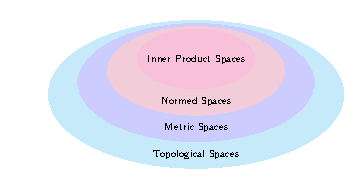
\includegraphics[scale=2]{doc/structure_spaces/structure_spaces.pdf}
	\caption{Overview of the generality of different spaces}
\end{figure}

\begin{theorem}{Pythagoral Theorem}{pyth_theo}
	Let $V$ be an Euclidean/Hermitian vector space and $u, v \in V$ with $u \perp v$. Then 
	\[
		\Vert u + v \Vert ^2 = \Vert u \Vert ^2 + \Vert v \Vert ^2.
	\]
\end{theorem}




	
	
	
	
\end{document}
